% Options for packages loaded elsewhere
\PassOptionsToPackage{unicode}{hyperref}
\PassOptionsToPackage{hyphens}{url}
%
\documentclass[
  ignorenonframetext,
]{beamer}
\usepackage{pgfpages}
\setbeamertemplate{caption}[numbered]
\setbeamertemplate{caption label separator}{: }
\setbeamercolor{caption name}{fg=normal text.fg}
\beamertemplatenavigationsymbolsempty
% Prevent slide breaks in the middle of a paragraph
\widowpenalties 1 10000
\raggedbottom
\setbeamertemplate{part page}{
  \centering
  \begin{beamercolorbox}[sep=16pt,center]{part title}
    \usebeamerfont{part title}\insertpart\par
  \end{beamercolorbox}
}
\setbeamertemplate{section page}{
  \centering
  \begin{beamercolorbox}[sep=12pt,center]{part title}
    \usebeamerfont{section title}\insertsection\par
  \end{beamercolorbox}
}
\setbeamertemplate{subsection page}{
  \centering
  \begin{beamercolorbox}[sep=8pt,center]{part title}
    \usebeamerfont{subsection title}\insertsubsection\par
  \end{beamercolorbox}
}
\AtBeginPart{
  \frame{\partpage}
}
\AtBeginSection{
  \ifbibliography
  \else
    \frame{\sectionpage}
  \fi
}
\AtBeginSubsection{
  \frame{\subsectionpage}
}
\usepackage{amsmath,amssymb}
\usepackage{iftex}
\ifPDFTeX
  \usepackage[T1]{fontenc}
  \usepackage[utf8]{inputenc}
  \usepackage{textcomp} % provide euro and other symbols
\else % if luatex or xetex
  \usepackage{unicode-math} % this also loads fontspec
  \defaultfontfeatures{Scale=MatchLowercase}
  \defaultfontfeatures[\rmfamily]{Ligatures=TeX,Scale=1}
\fi
\usepackage{lmodern}
\usetheme[]{metropolis}
\usecolortheme{seahorse}
\ifPDFTeX\else
  % xetex/luatex font selection
\fi
% Use upquote if available, for straight quotes in verbatim environments
\IfFileExists{upquote.sty}{\usepackage{upquote}}{}
\IfFileExists{microtype.sty}{% use microtype if available
  \usepackage[]{microtype}
  \UseMicrotypeSet[protrusion]{basicmath} % disable protrusion for tt fonts
}{}
\makeatletter
\@ifundefined{KOMAClassName}{% if non-KOMA class
  \IfFileExists{parskip.sty}{%
    \usepackage{parskip}
  }{% else
    \setlength{\parindent}{0pt}
    \setlength{\parskip}{6pt plus 2pt minus 1pt}}
}{% if KOMA class
  \KOMAoptions{parskip=half}}
\makeatother
\usepackage{xcolor}
\newif\ifbibliography
\usepackage{graphicx}
\makeatletter
\newsavebox\pandoc@box
\newcommand*\pandocbounded[1]{% scales image to fit in text height/width
  \sbox\pandoc@box{#1}%
  \Gscale@div\@tempa{\textheight}{\dimexpr\ht\pandoc@box+\dp\pandoc@box\relax}%
  \Gscale@div\@tempb{\linewidth}{\wd\pandoc@box}%
  \ifdim\@tempb\p@<\@tempa\p@\let\@tempa\@tempb\fi% select the smaller of both
  \ifdim\@tempa\p@<\p@\scalebox{\@tempa}{\usebox\pandoc@box}%
  \else\usebox{\pandoc@box}%
  \fi%
}
% Set default figure placement to htbp
\def\fps@figure{htbp}
\makeatother
\setlength{\emergencystretch}{3em} % prevent overfull lines
\providecommand{\tightlist}{%
  \setlength{\itemsep}{0pt}\setlength{\parskip}{0pt}}
\setcounter{secnumdepth}{-\maxdimen} % remove section numbering
\usepackage{xcolor}
\definecolor{myorange}{RGB}{255, 94, 77}
\setbeamertemplate{footline}{}
\usepackage{bookmark}
\IfFileExists{xurl.sty}{\usepackage{xurl}}{} % add URL line breaks if available
\urlstyle{same}
\hypersetup{
  pdftitle={Graphical Unexcellence},
  pdfauthor={(\textbackslash text\{Professor Dave\})\^{}2},
  hidelinks,
  pdfcreator={LaTeX via pandoc}}

\title{Graphical Unexcellence}
\subtitle{Data Viz Hall of Shame}
\author{\((\text{Professor Dave})^2\)}
\date{}
\institute{The University of Austin}

\begin{document}
\frame{\titlepage}

\begin{frame}{Outline}
\phantomsection\label{outline}
\begin{itemize}
\tightlist
\item
  Plotting pitfalls: Hall of shame
\item
  Plot critiques
\item
  The grammar of graphics
\item
  The five most important plots
\item
  Enriching plots (color, faceting, labels, etc)
\end{itemize}
\end{frame}

\begin{frame}{Plotting pitfalls}
\phantomsection\label{plotting-pitfalls}
\begin{itemize}
\tightlist
\item
  \textcolor{orange}{Axis trickery (a.k.a. “little y lies”)}
\item
  Violations of basic math
\item
  Nearly content-free figures
\item
  Gratuitous chartjunk
\item
  Poorly chosen 3D graphics
\item
  Bad design choices
\end{itemize}
\end{frame}

\begin{frame}{}
\phantomsection\label{section}
\pandocbounded{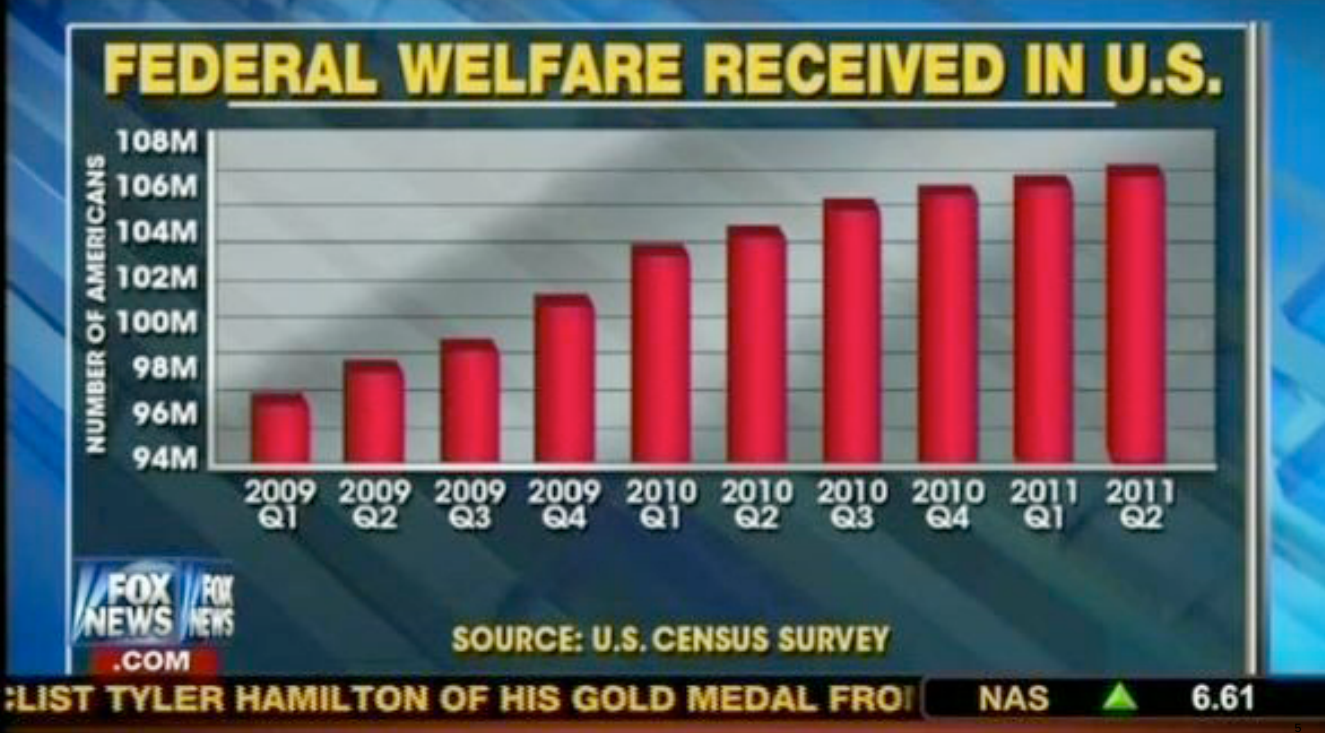
\includegraphics[keepaspectratio]{hallofshame_figs/fig_5.png}}
\end{frame}

\begin{frame}{}
\phantomsection\label{section-1}
\pandocbounded{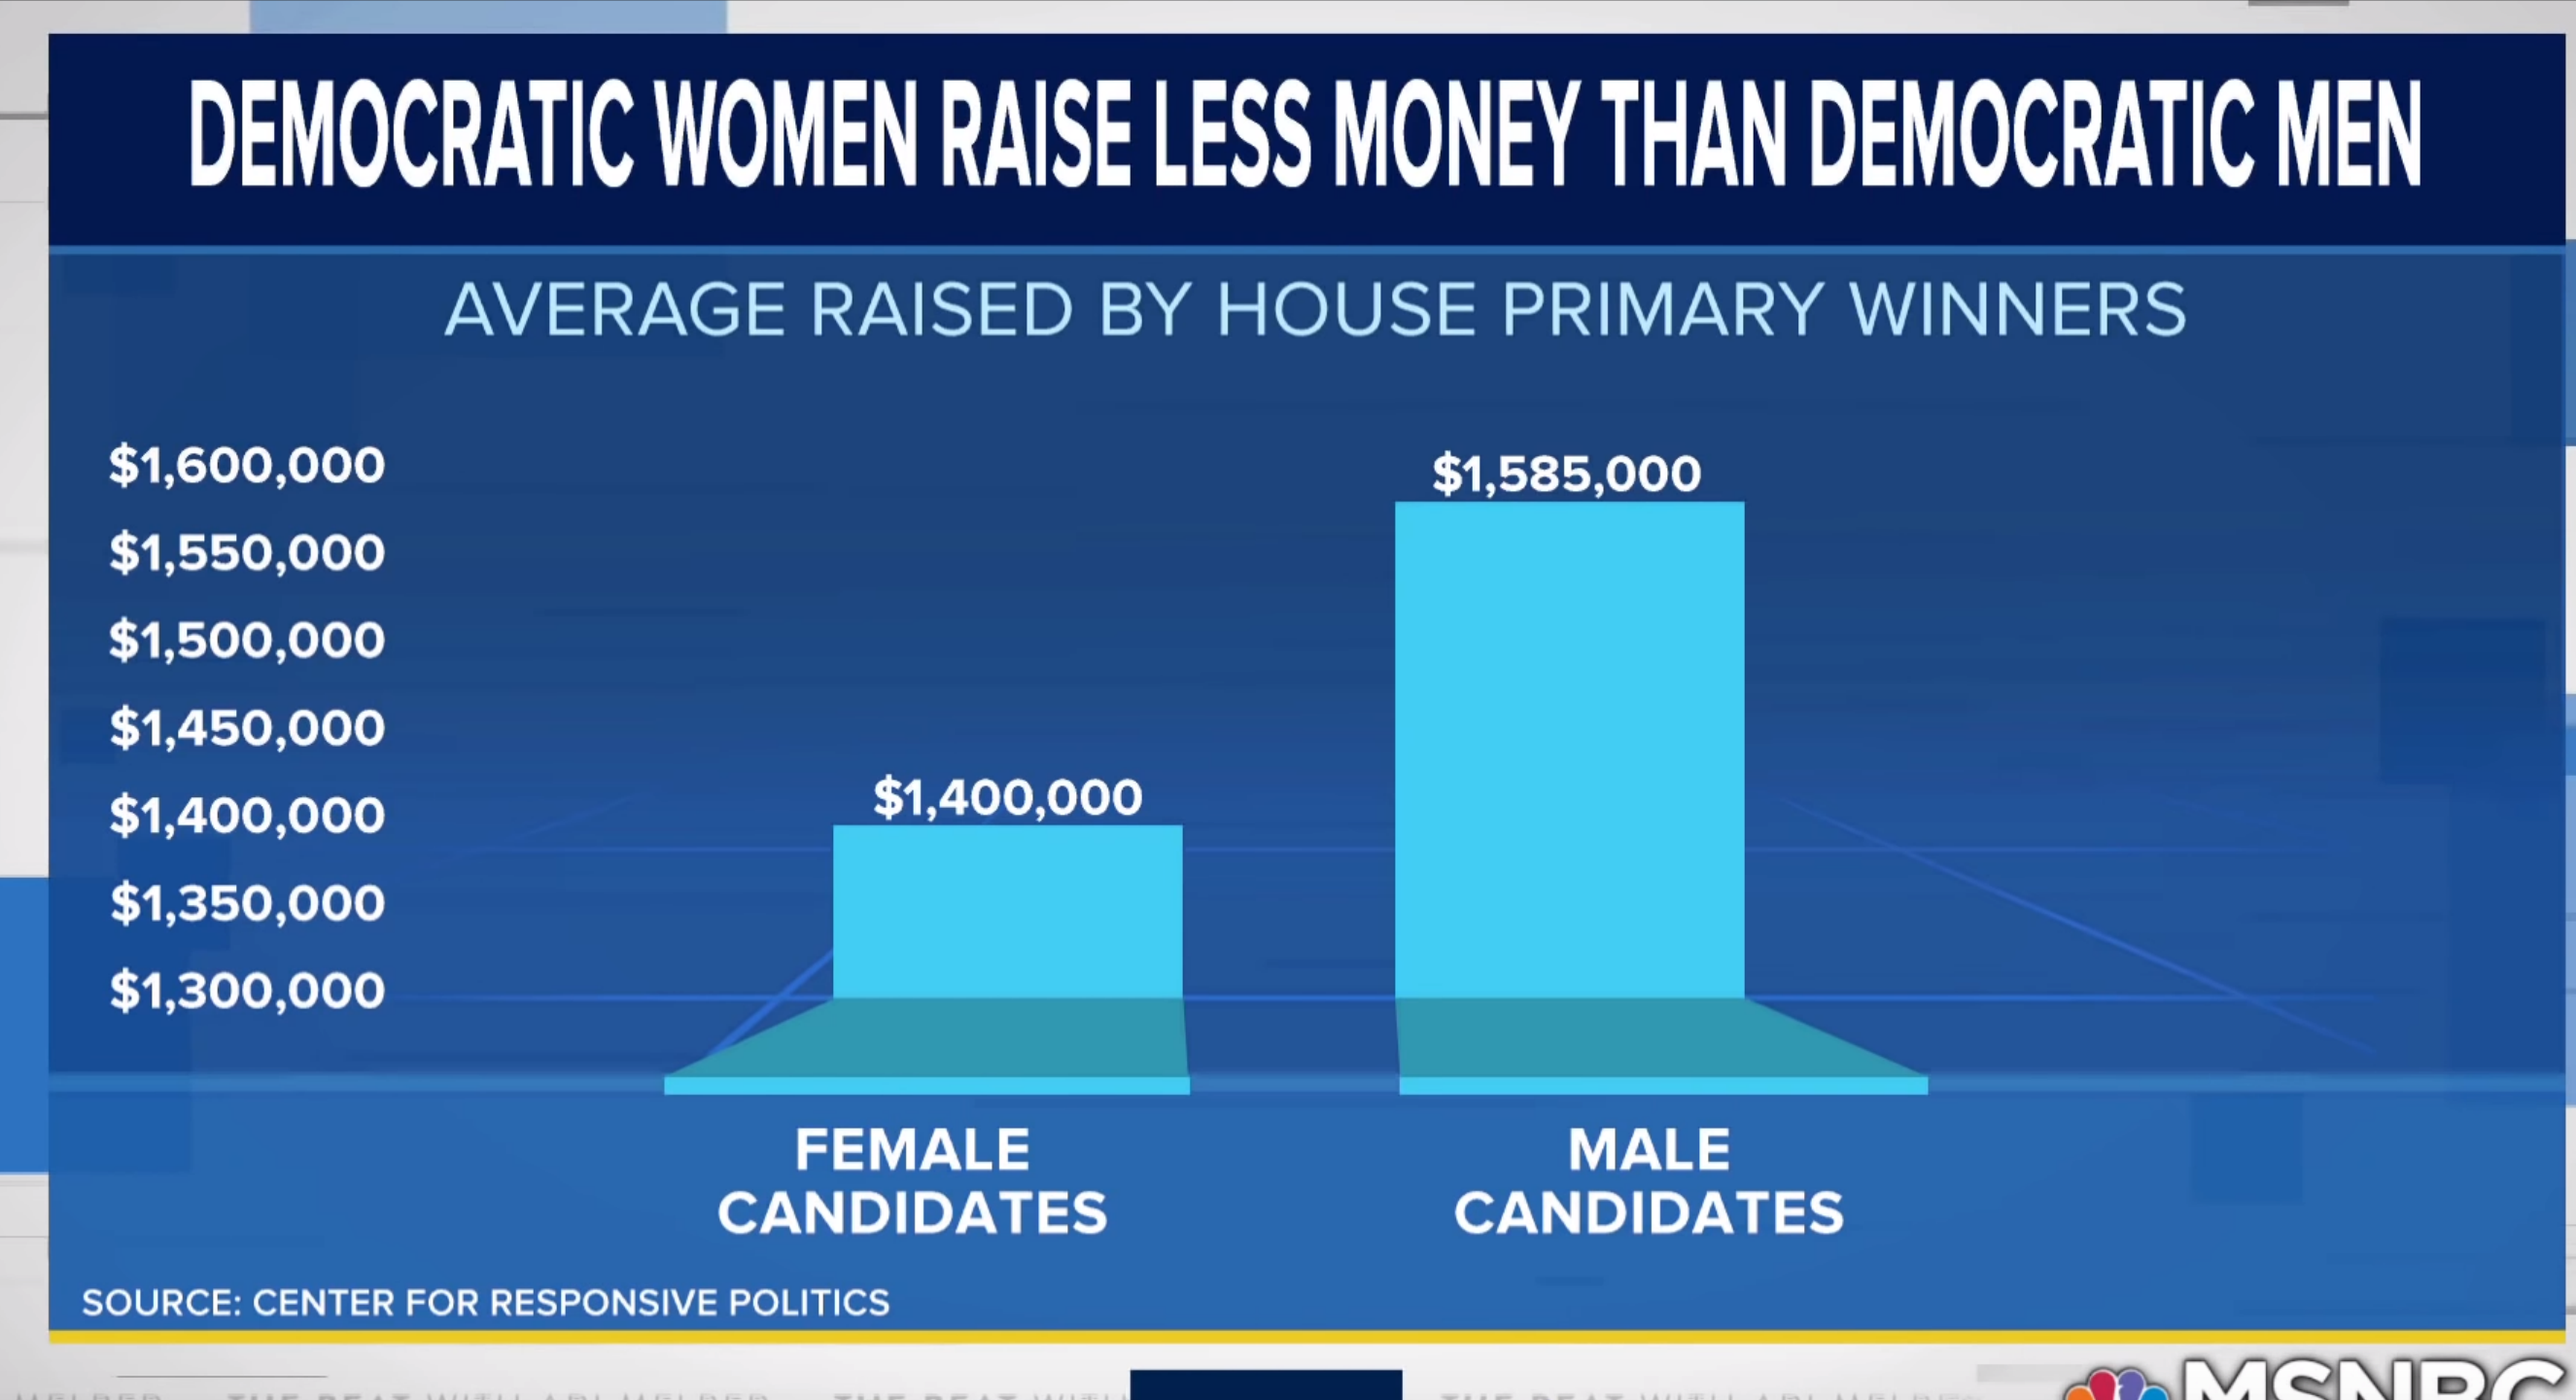
\includegraphics[keepaspectratio]{hallofshame_figs/fig_6.png}}
\end{frame}

\begin{frame}{}
\phantomsection\label{section-2}
\pandocbounded{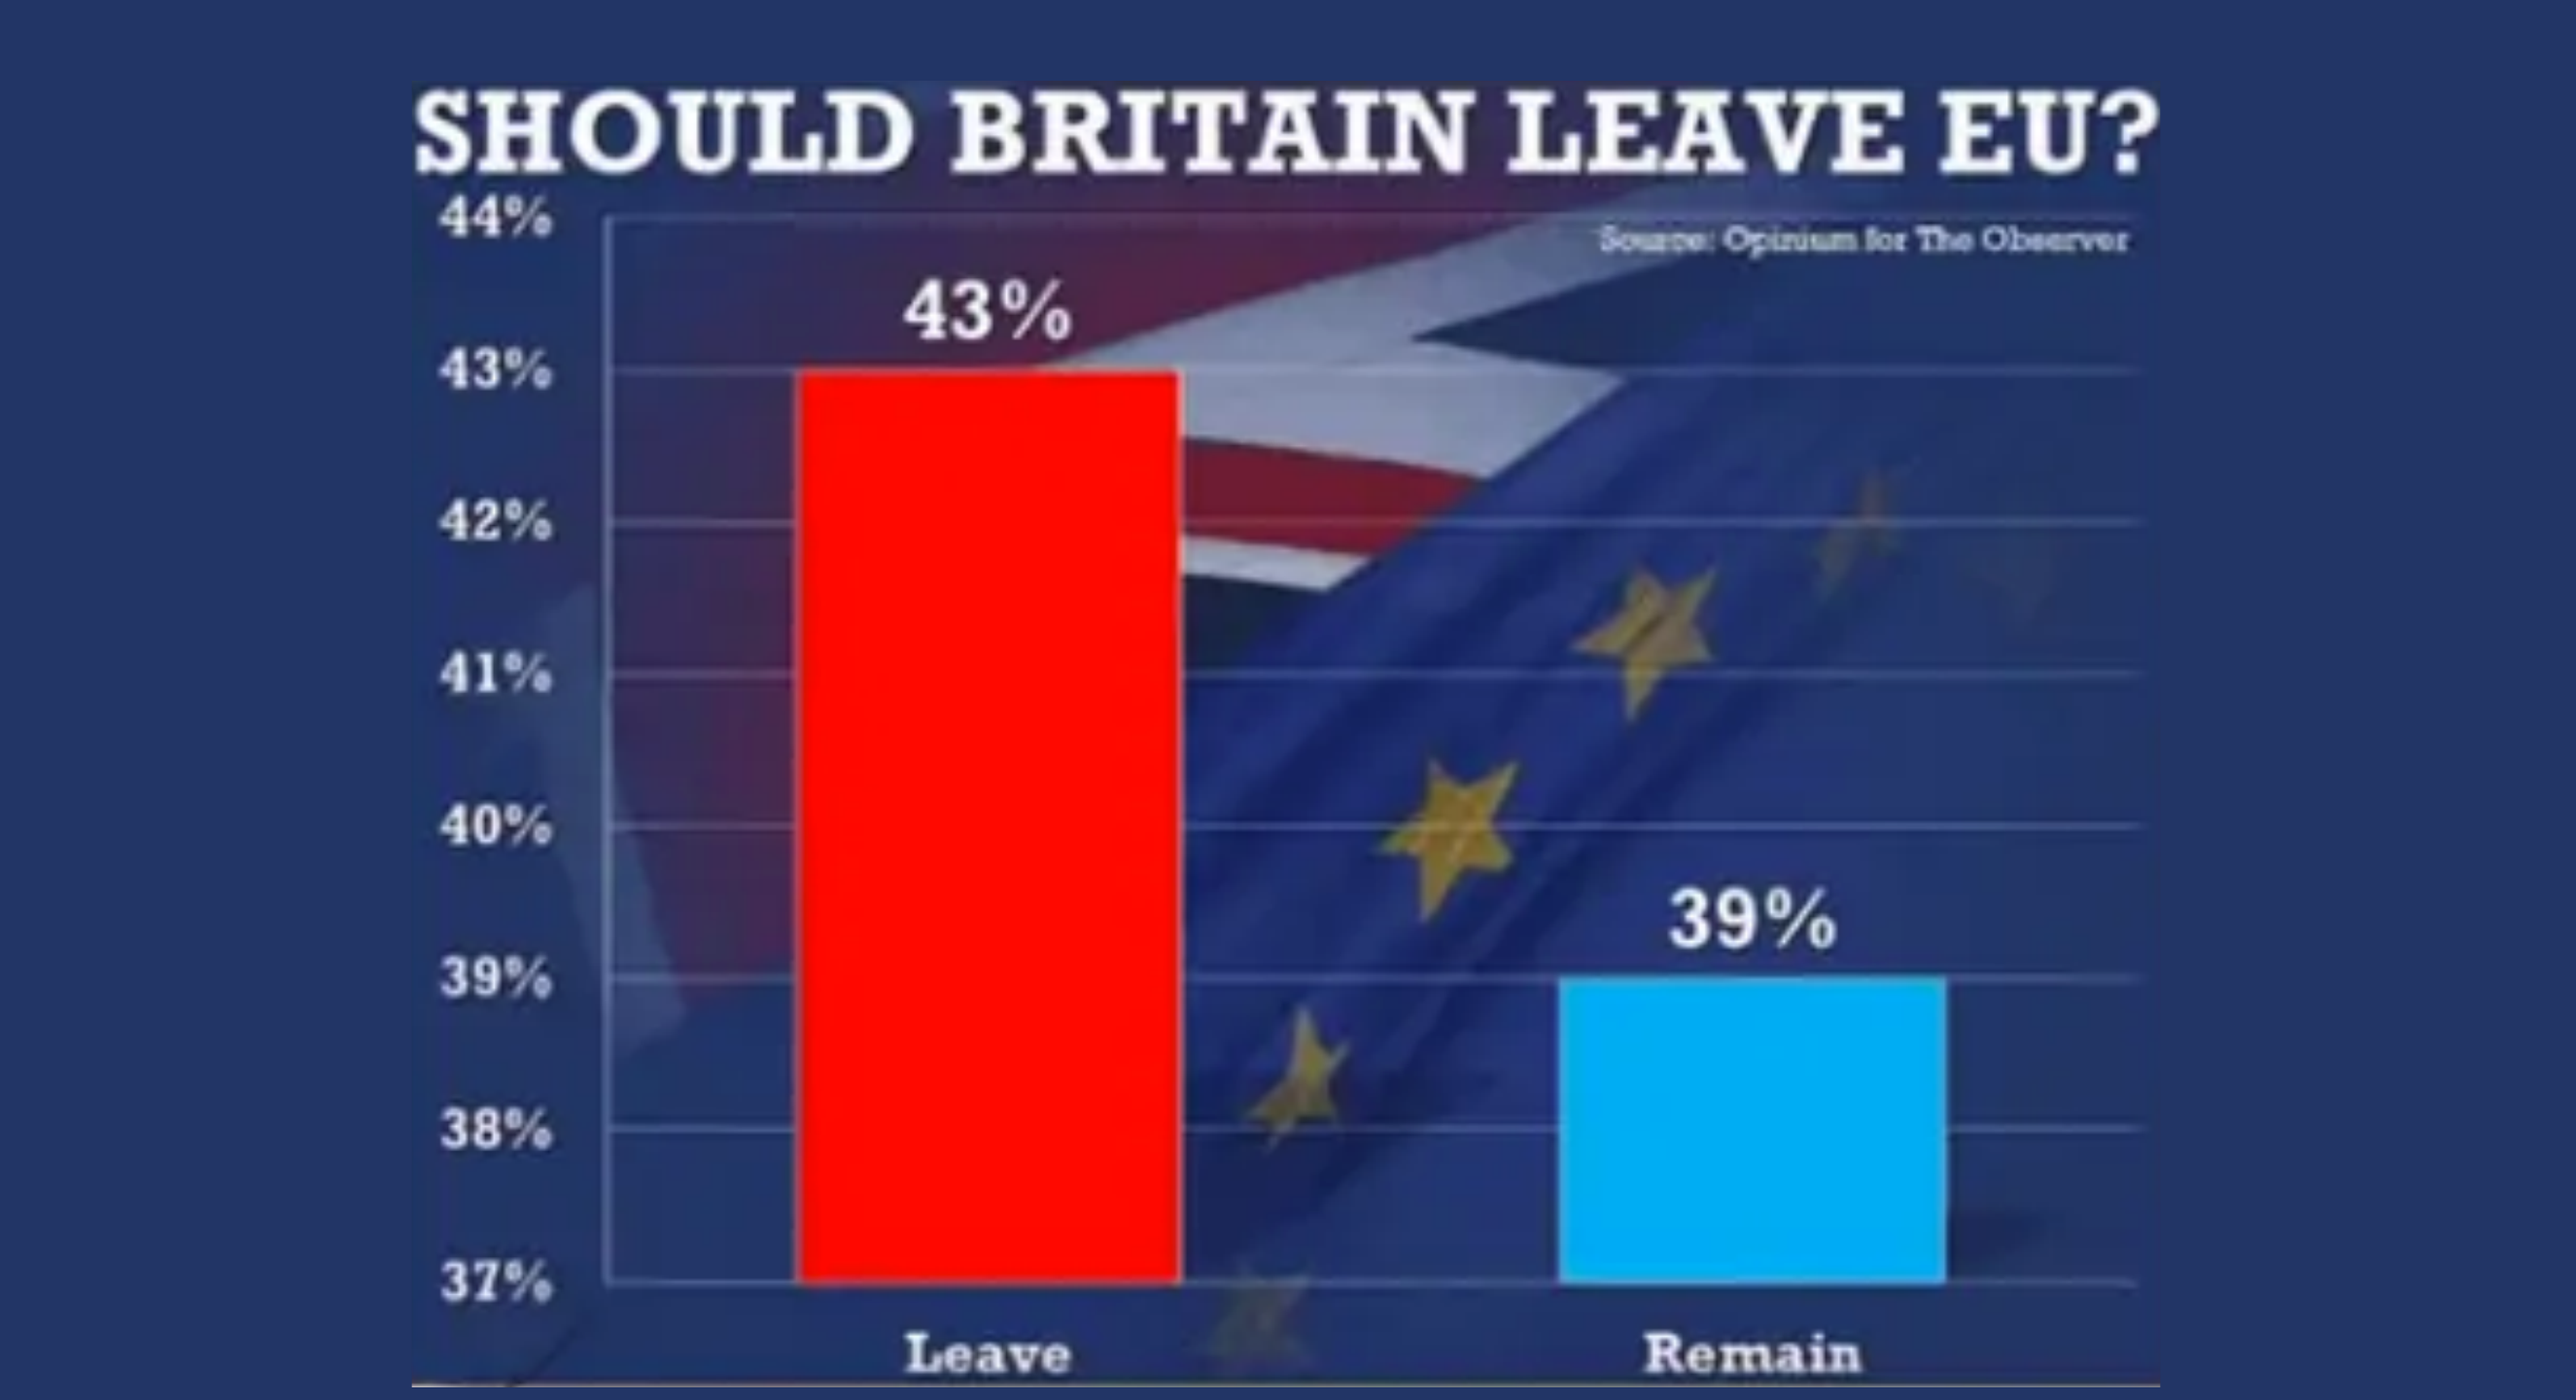
\includegraphics[keepaspectratio]{hallofshame_figs/fig_7.png}}
\end{frame}

\begin{frame}{}
\phantomsection\label{section-3}
\pandocbounded{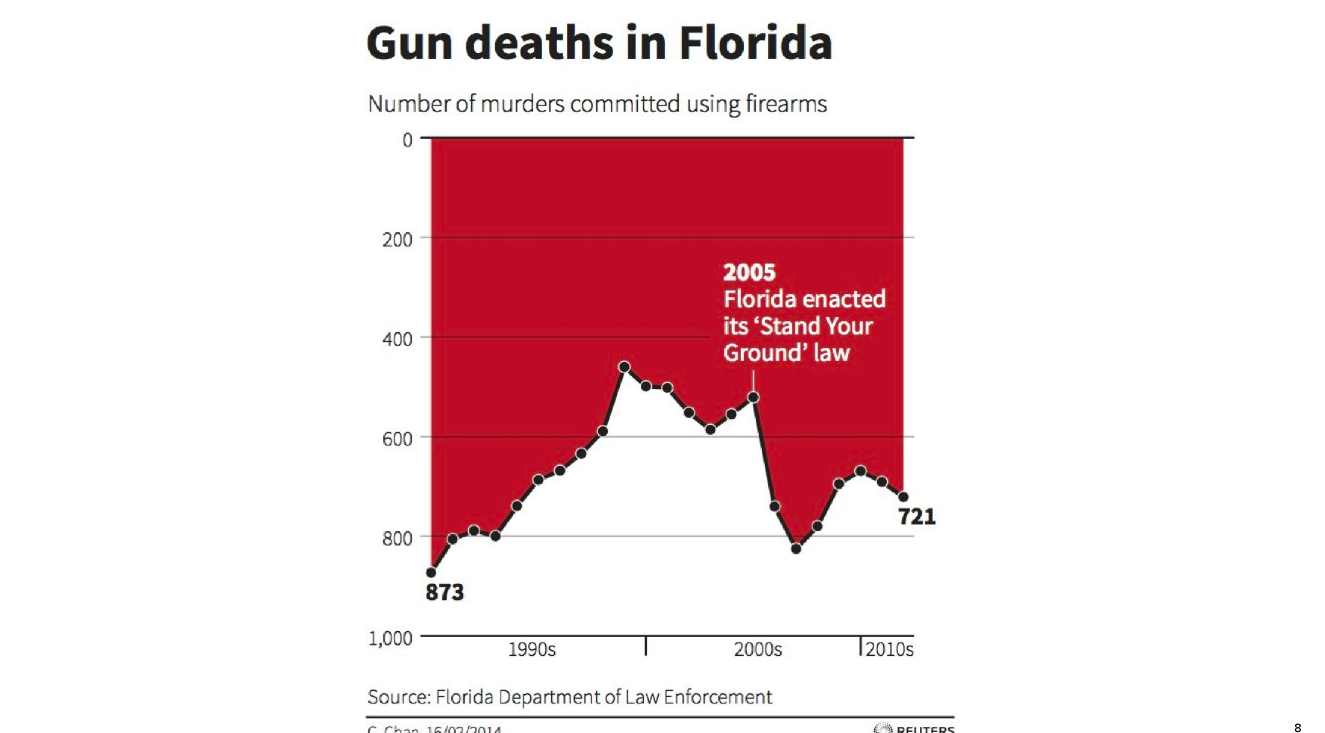
\includegraphics[keepaspectratio]{hallofshame_figs/fig_8.png}}
\end{frame}

\begin{frame}{}
\phantomsection\label{section-4}
\centering

\huge \textbf{And yet \ldots{}}
\end{frame}

\begin{frame}{}
\phantomsection\label{section-5}
\pandocbounded{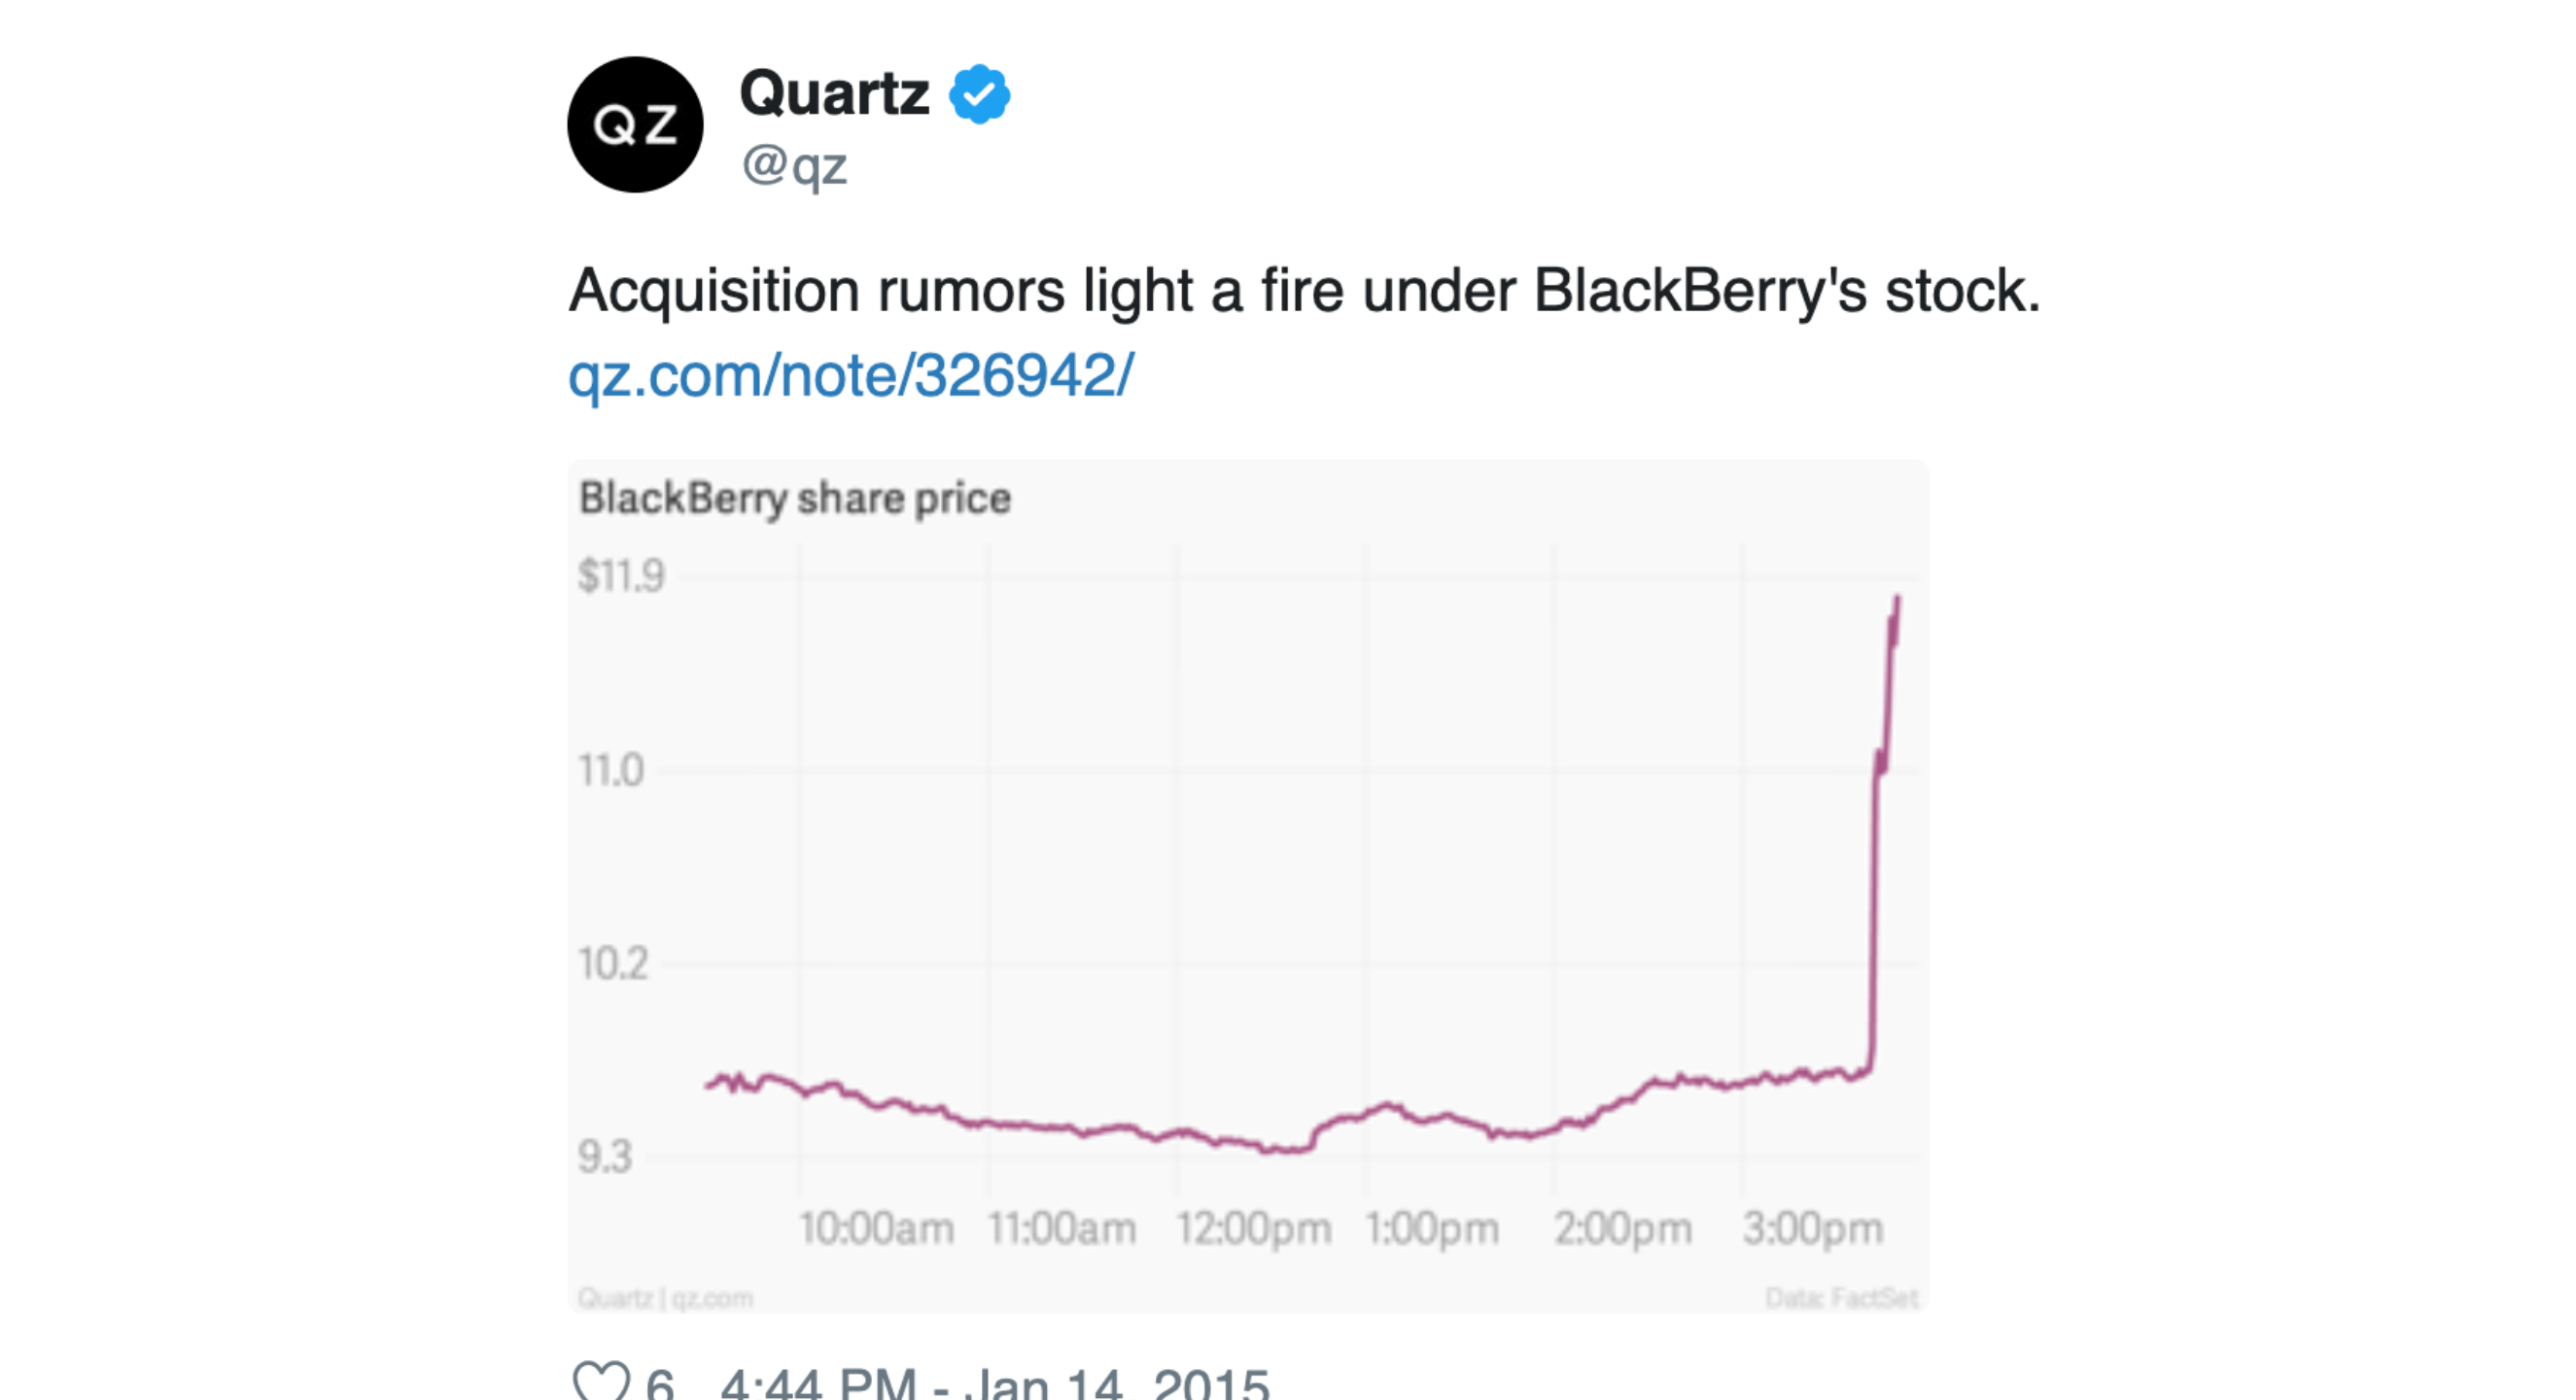
\includegraphics[keepaspectratio]{hallofshame_figs/fig_10.png}}
\end{frame}

\begin{frame}{}
\phantomsection\label{section-6}
\pandocbounded{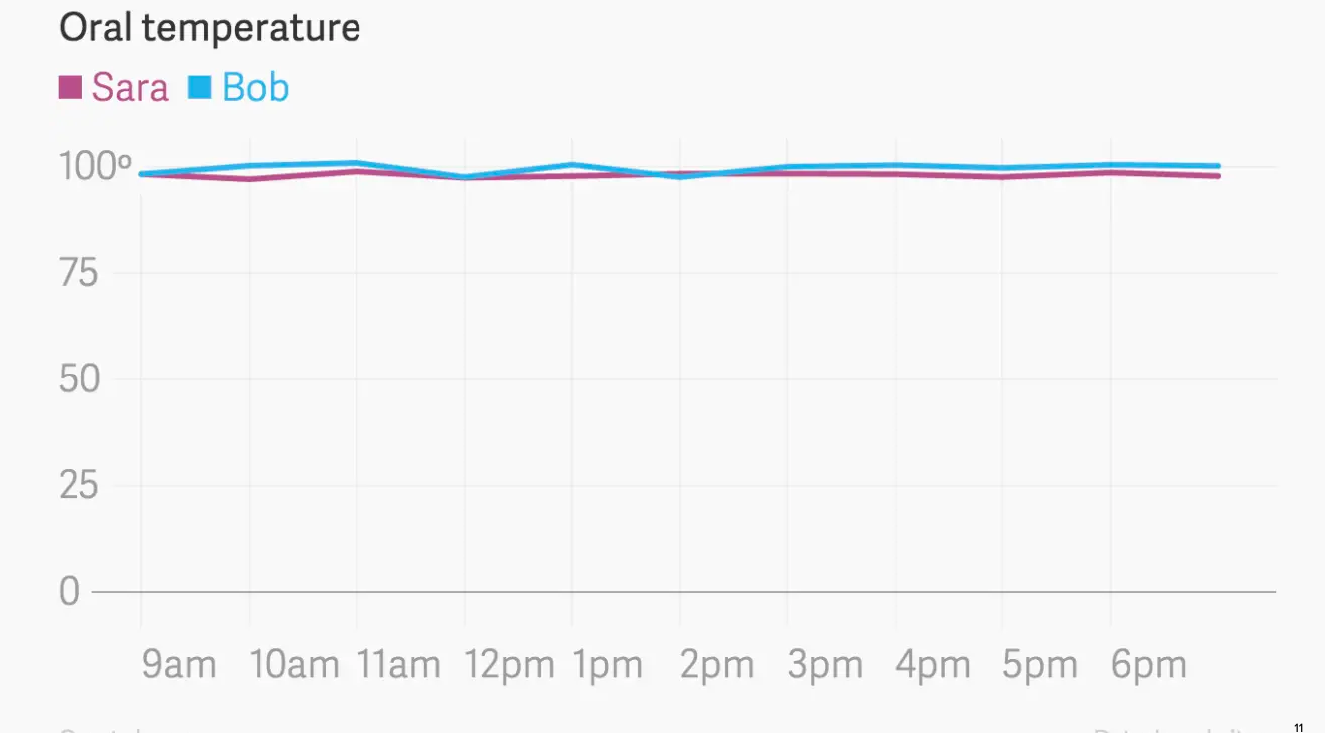
\includegraphics[keepaspectratio]{hallofshame_figs/fig_11.png}}
\end{frame}

\begin{frame}{}
\phantomsection\label{section-7}
\pandocbounded{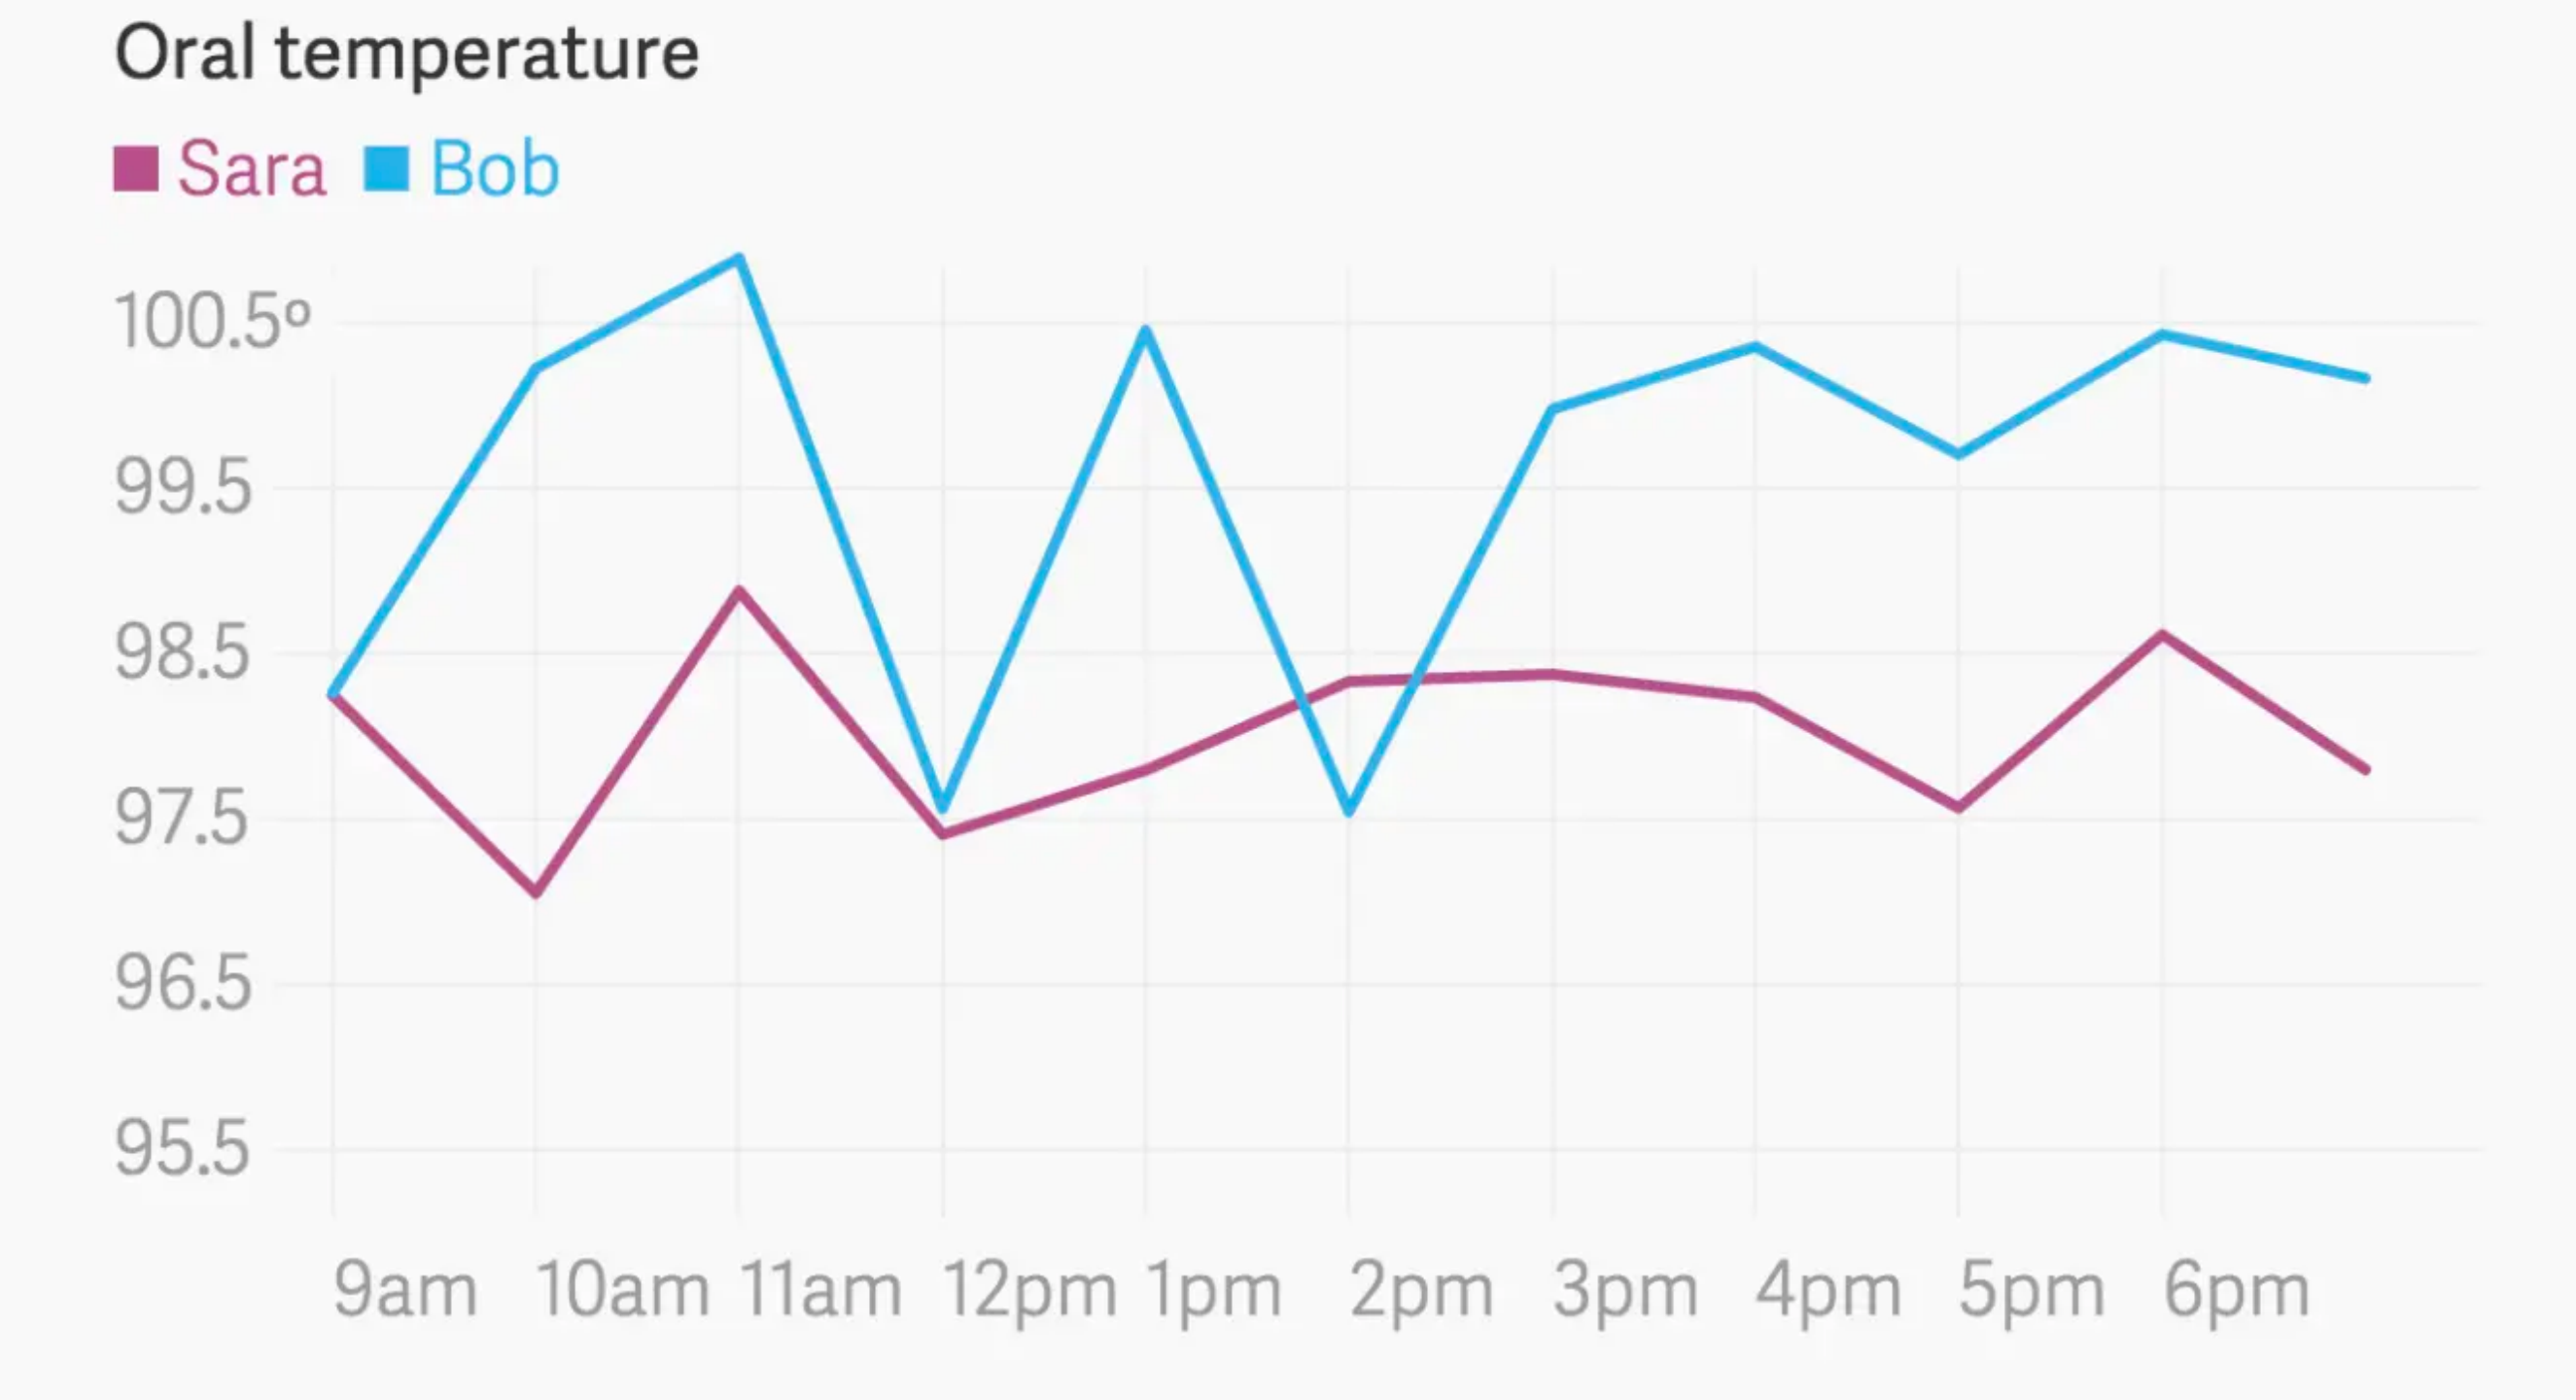
\includegraphics[keepaspectratio]{hallofshame_figs/fig_12.png}}
\end{frame}

\begin{frame}{Truncating the vertical axis is sometimes ok}
\phantomsection\label{truncating-the-vertical-axis-is-sometimes-ok}
\begin{itemize}
\tightlist
\item
  When you're trying to emphasize change, rather than relative
  magnitude.
\item
  When you're plotting data over time.
\item
  When zero is not a sensible baseline for comparison.
\end{itemize}

\textcolor{orange}{Bottom line} \ldots{} use your judgment; don't
mislead people; watch out for ``little y lies.''
\end{frame}

\begin{frame}{Plotting pitfalls}
\phantomsection\label{plotting-pitfalls-1}
\begin{itemize}
\tightlist
\item
  Axis trickery (a.k.a. ``little y lies'')
\item
  \textcolor{orange}{Violations of basic math}
\item
  Nearly content-free figures
\item
  Gratuitous chartjunk
\item
  Poorly chosen 3D graphics
\item
  Bad design choices
\end{itemize}
\end{frame}

\begin{frame}{}
\phantomsection\label{section-8}
\pandocbounded{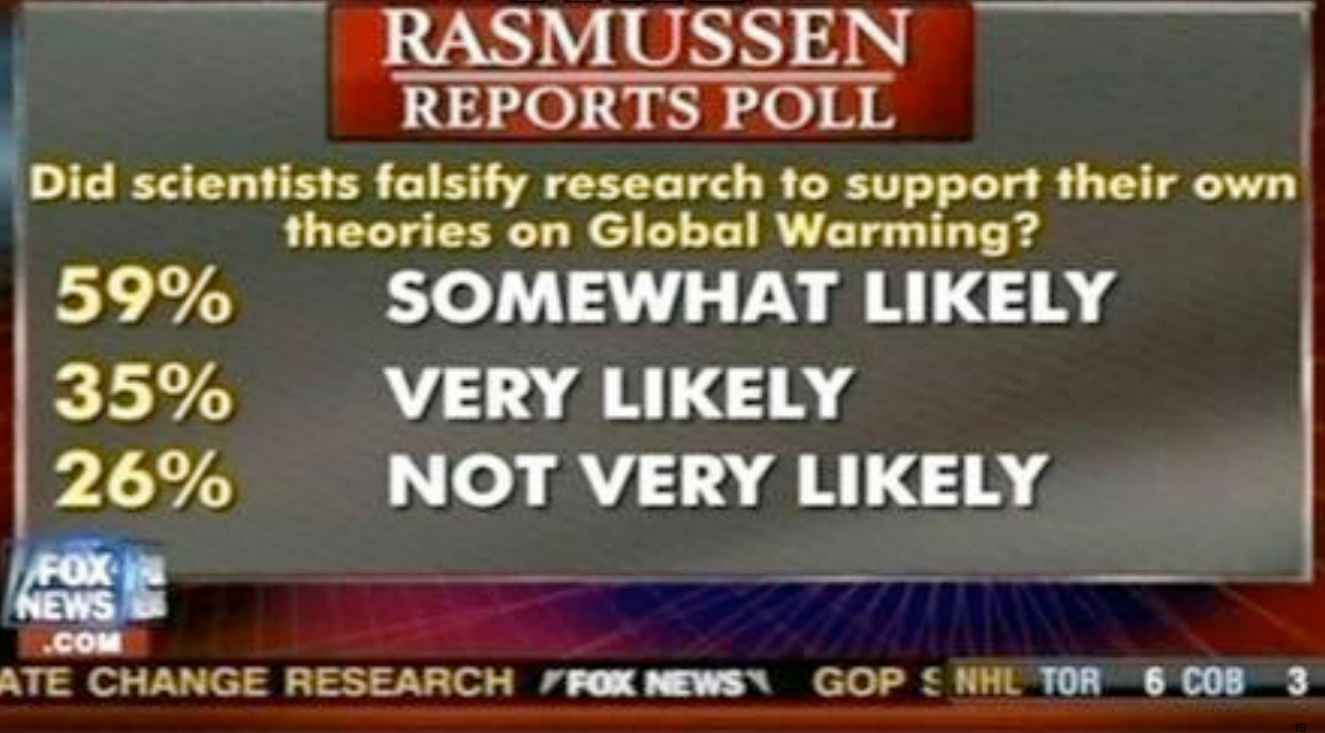
\includegraphics[keepaspectratio]{hallofshame_figs/fig_15.png}}
\end{frame}

\begin{frame}{}
\phantomsection\label{section-9}
\pandocbounded{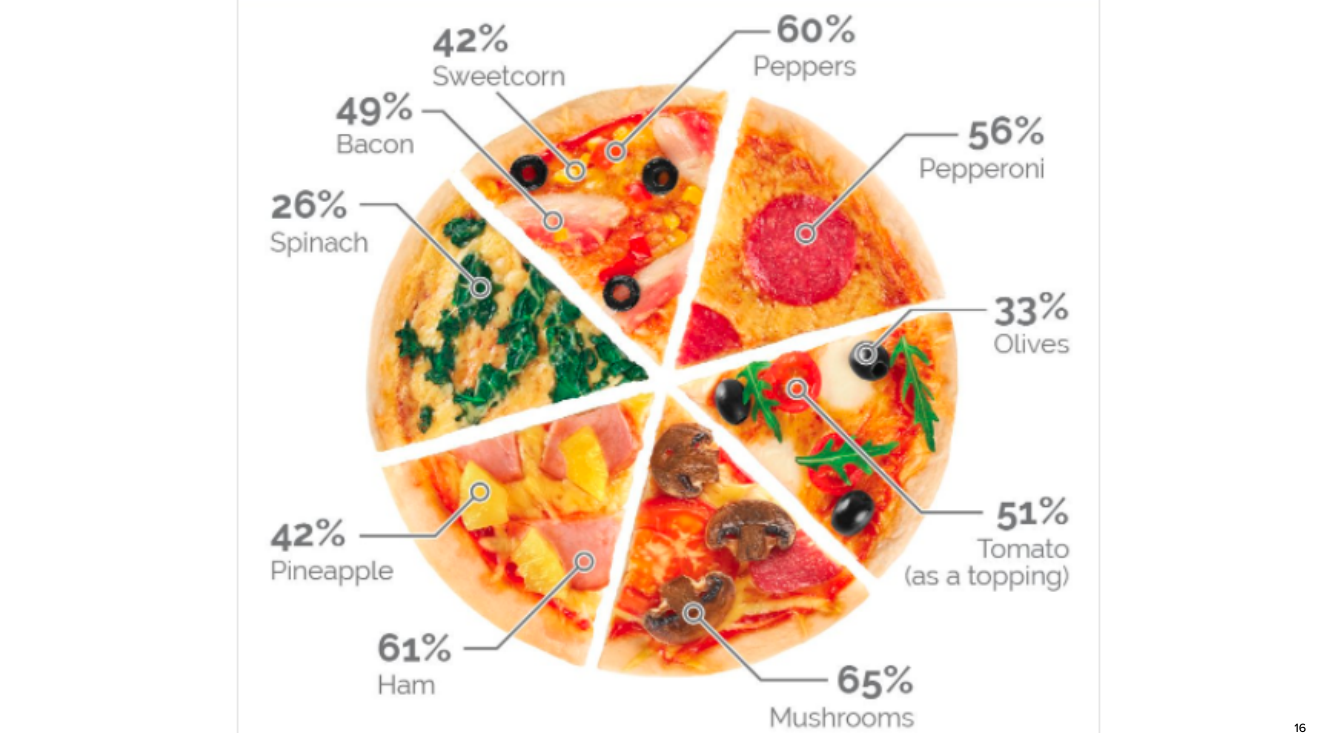
\includegraphics[keepaspectratio]{hallofshame_figs/fig_16.png}}
\end{frame}

\begin{frame}{}
\phantomsection\label{section-10}
\pandocbounded{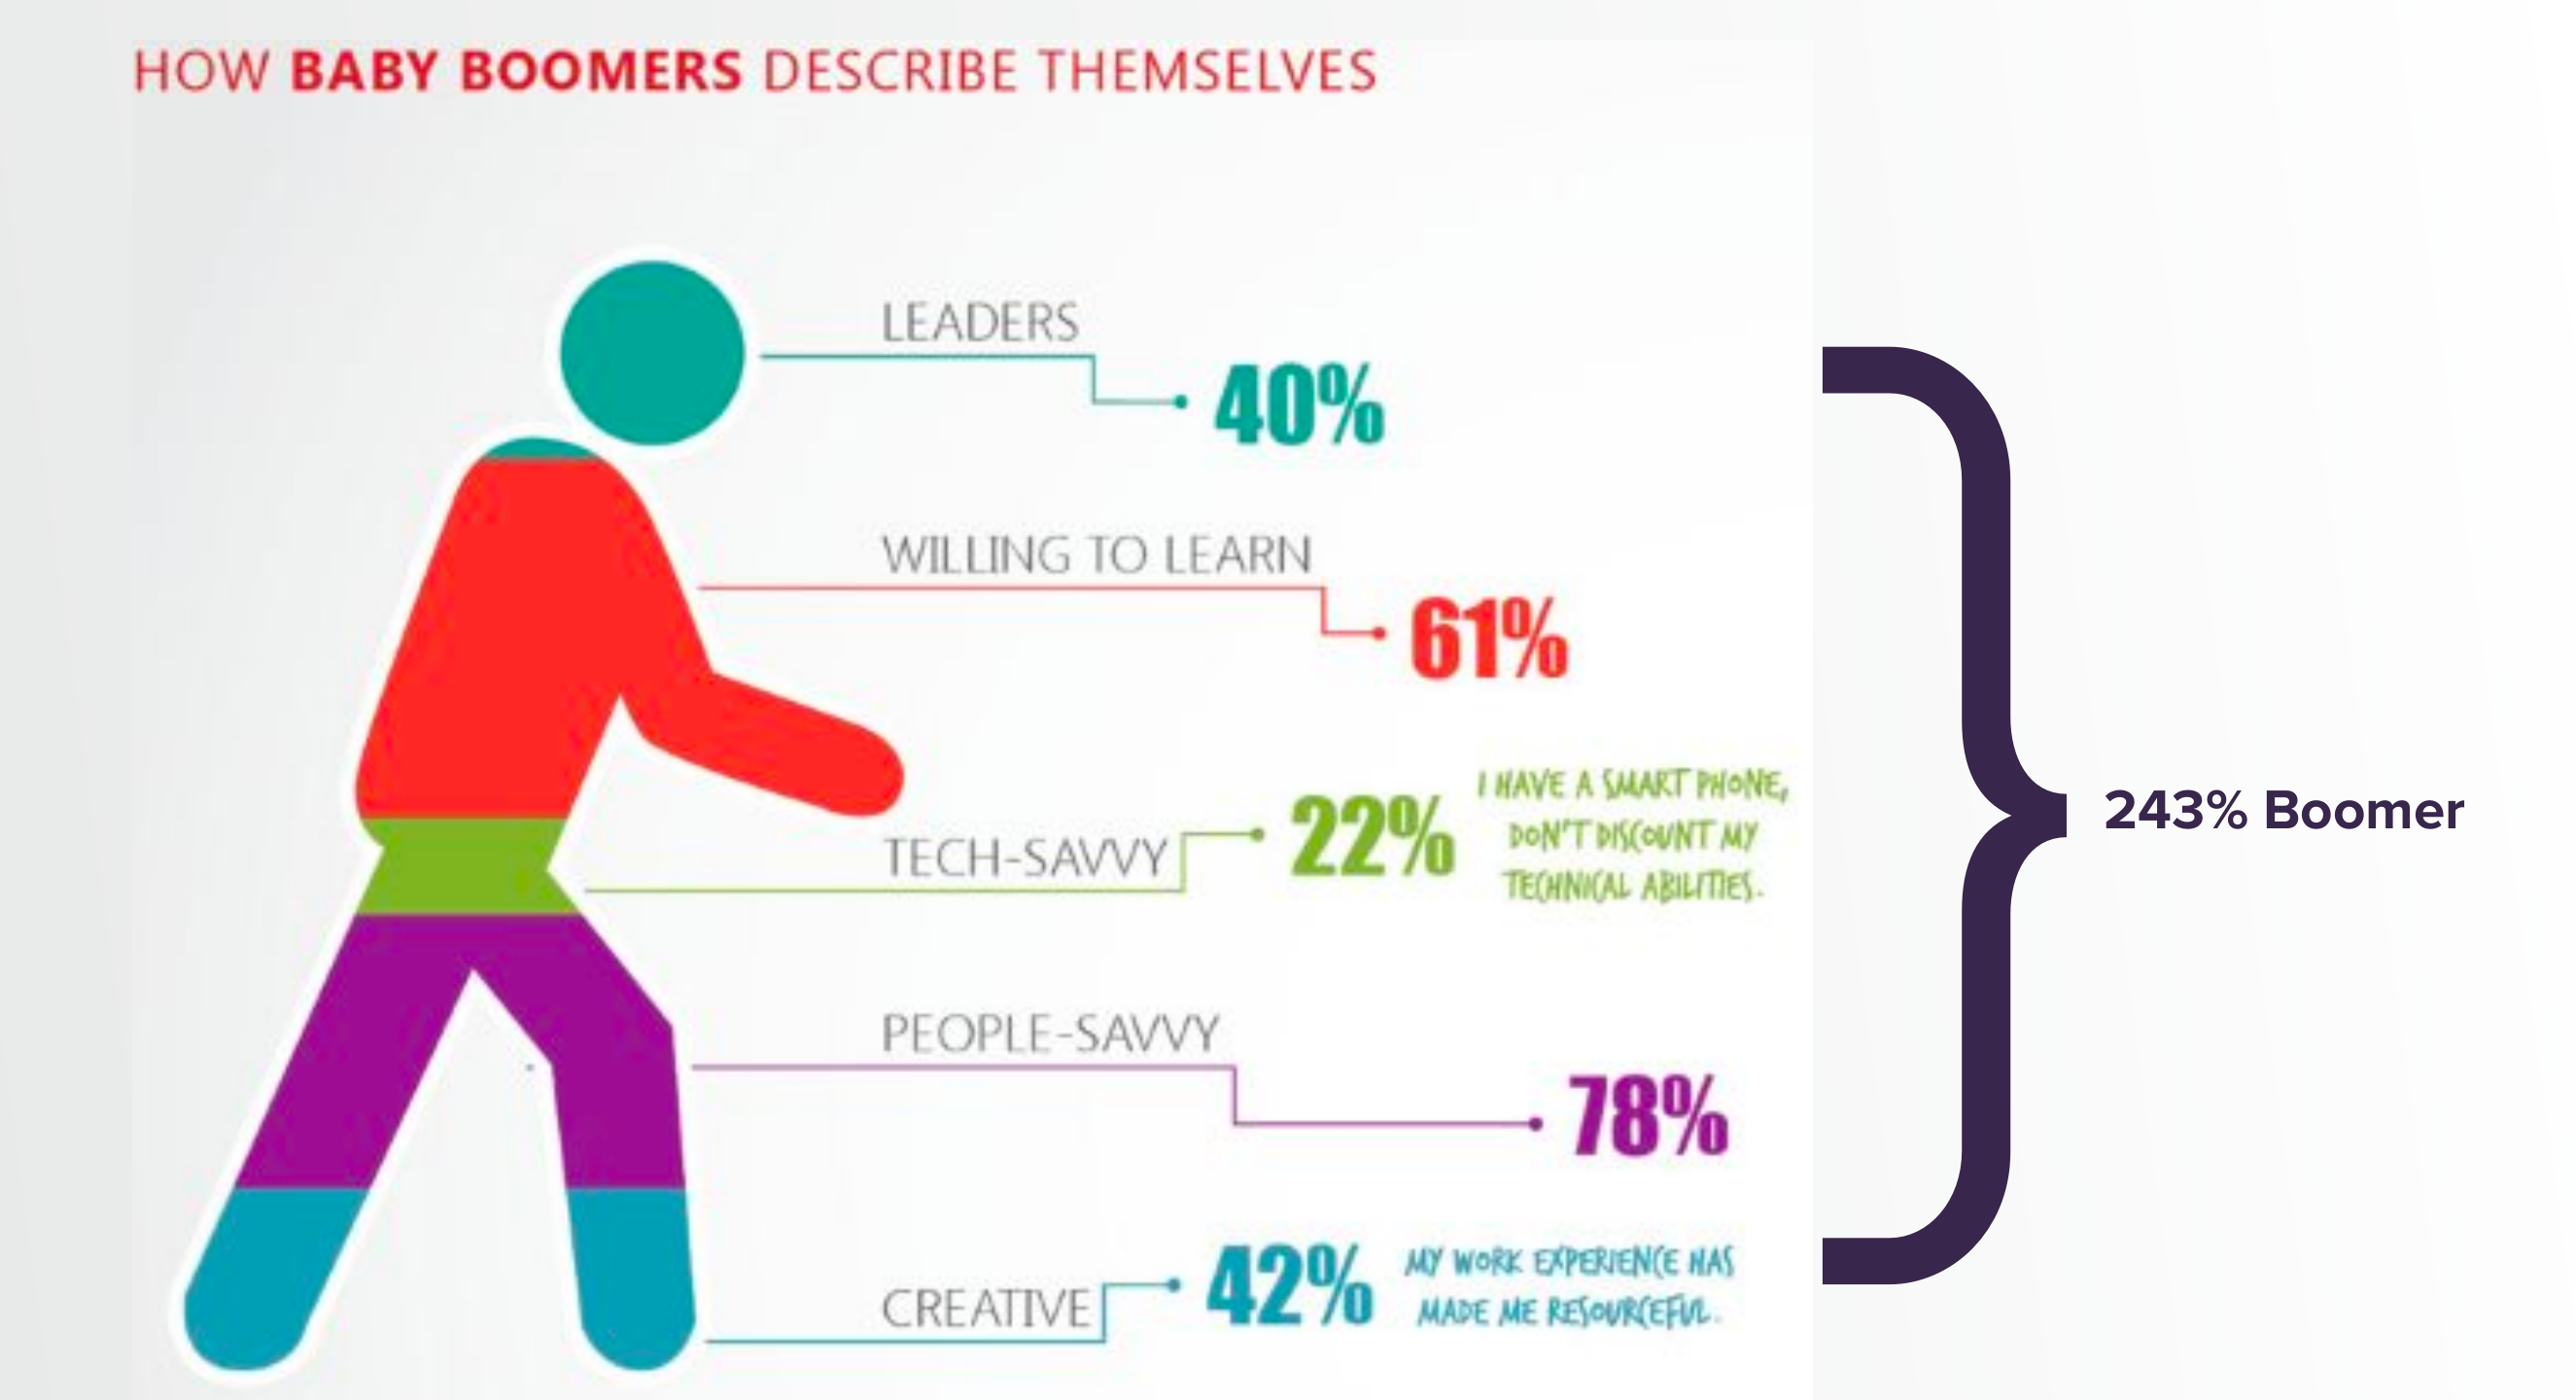
\includegraphics[keepaspectratio]{hallofshame_figs/fig_17.png}}
\end{frame}

\begin{frame}{}
\phantomsection\label{section-11}
\pandocbounded{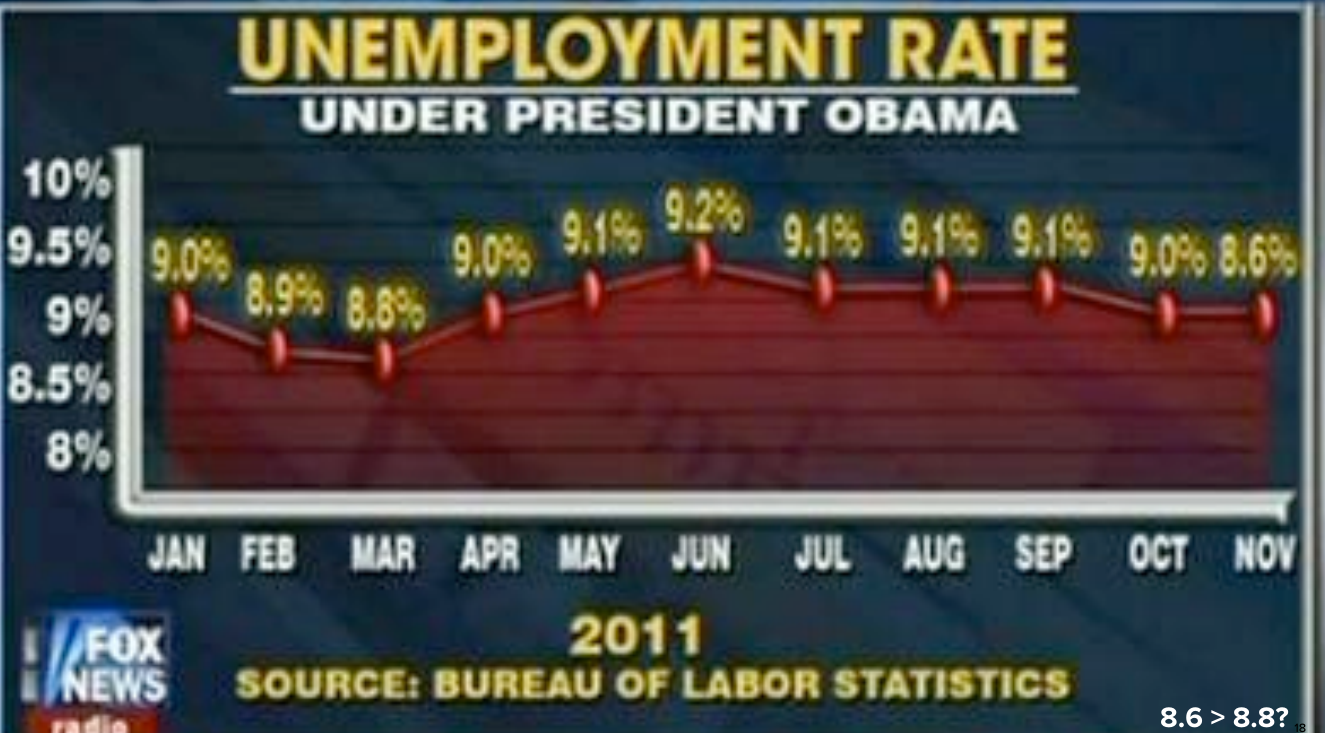
\includegraphics[keepaspectratio]{hallofshame_figs/fig_18.png}}
\end{frame}

\begin{frame}{}
\phantomsection\label{section-12}
\pandocbounded{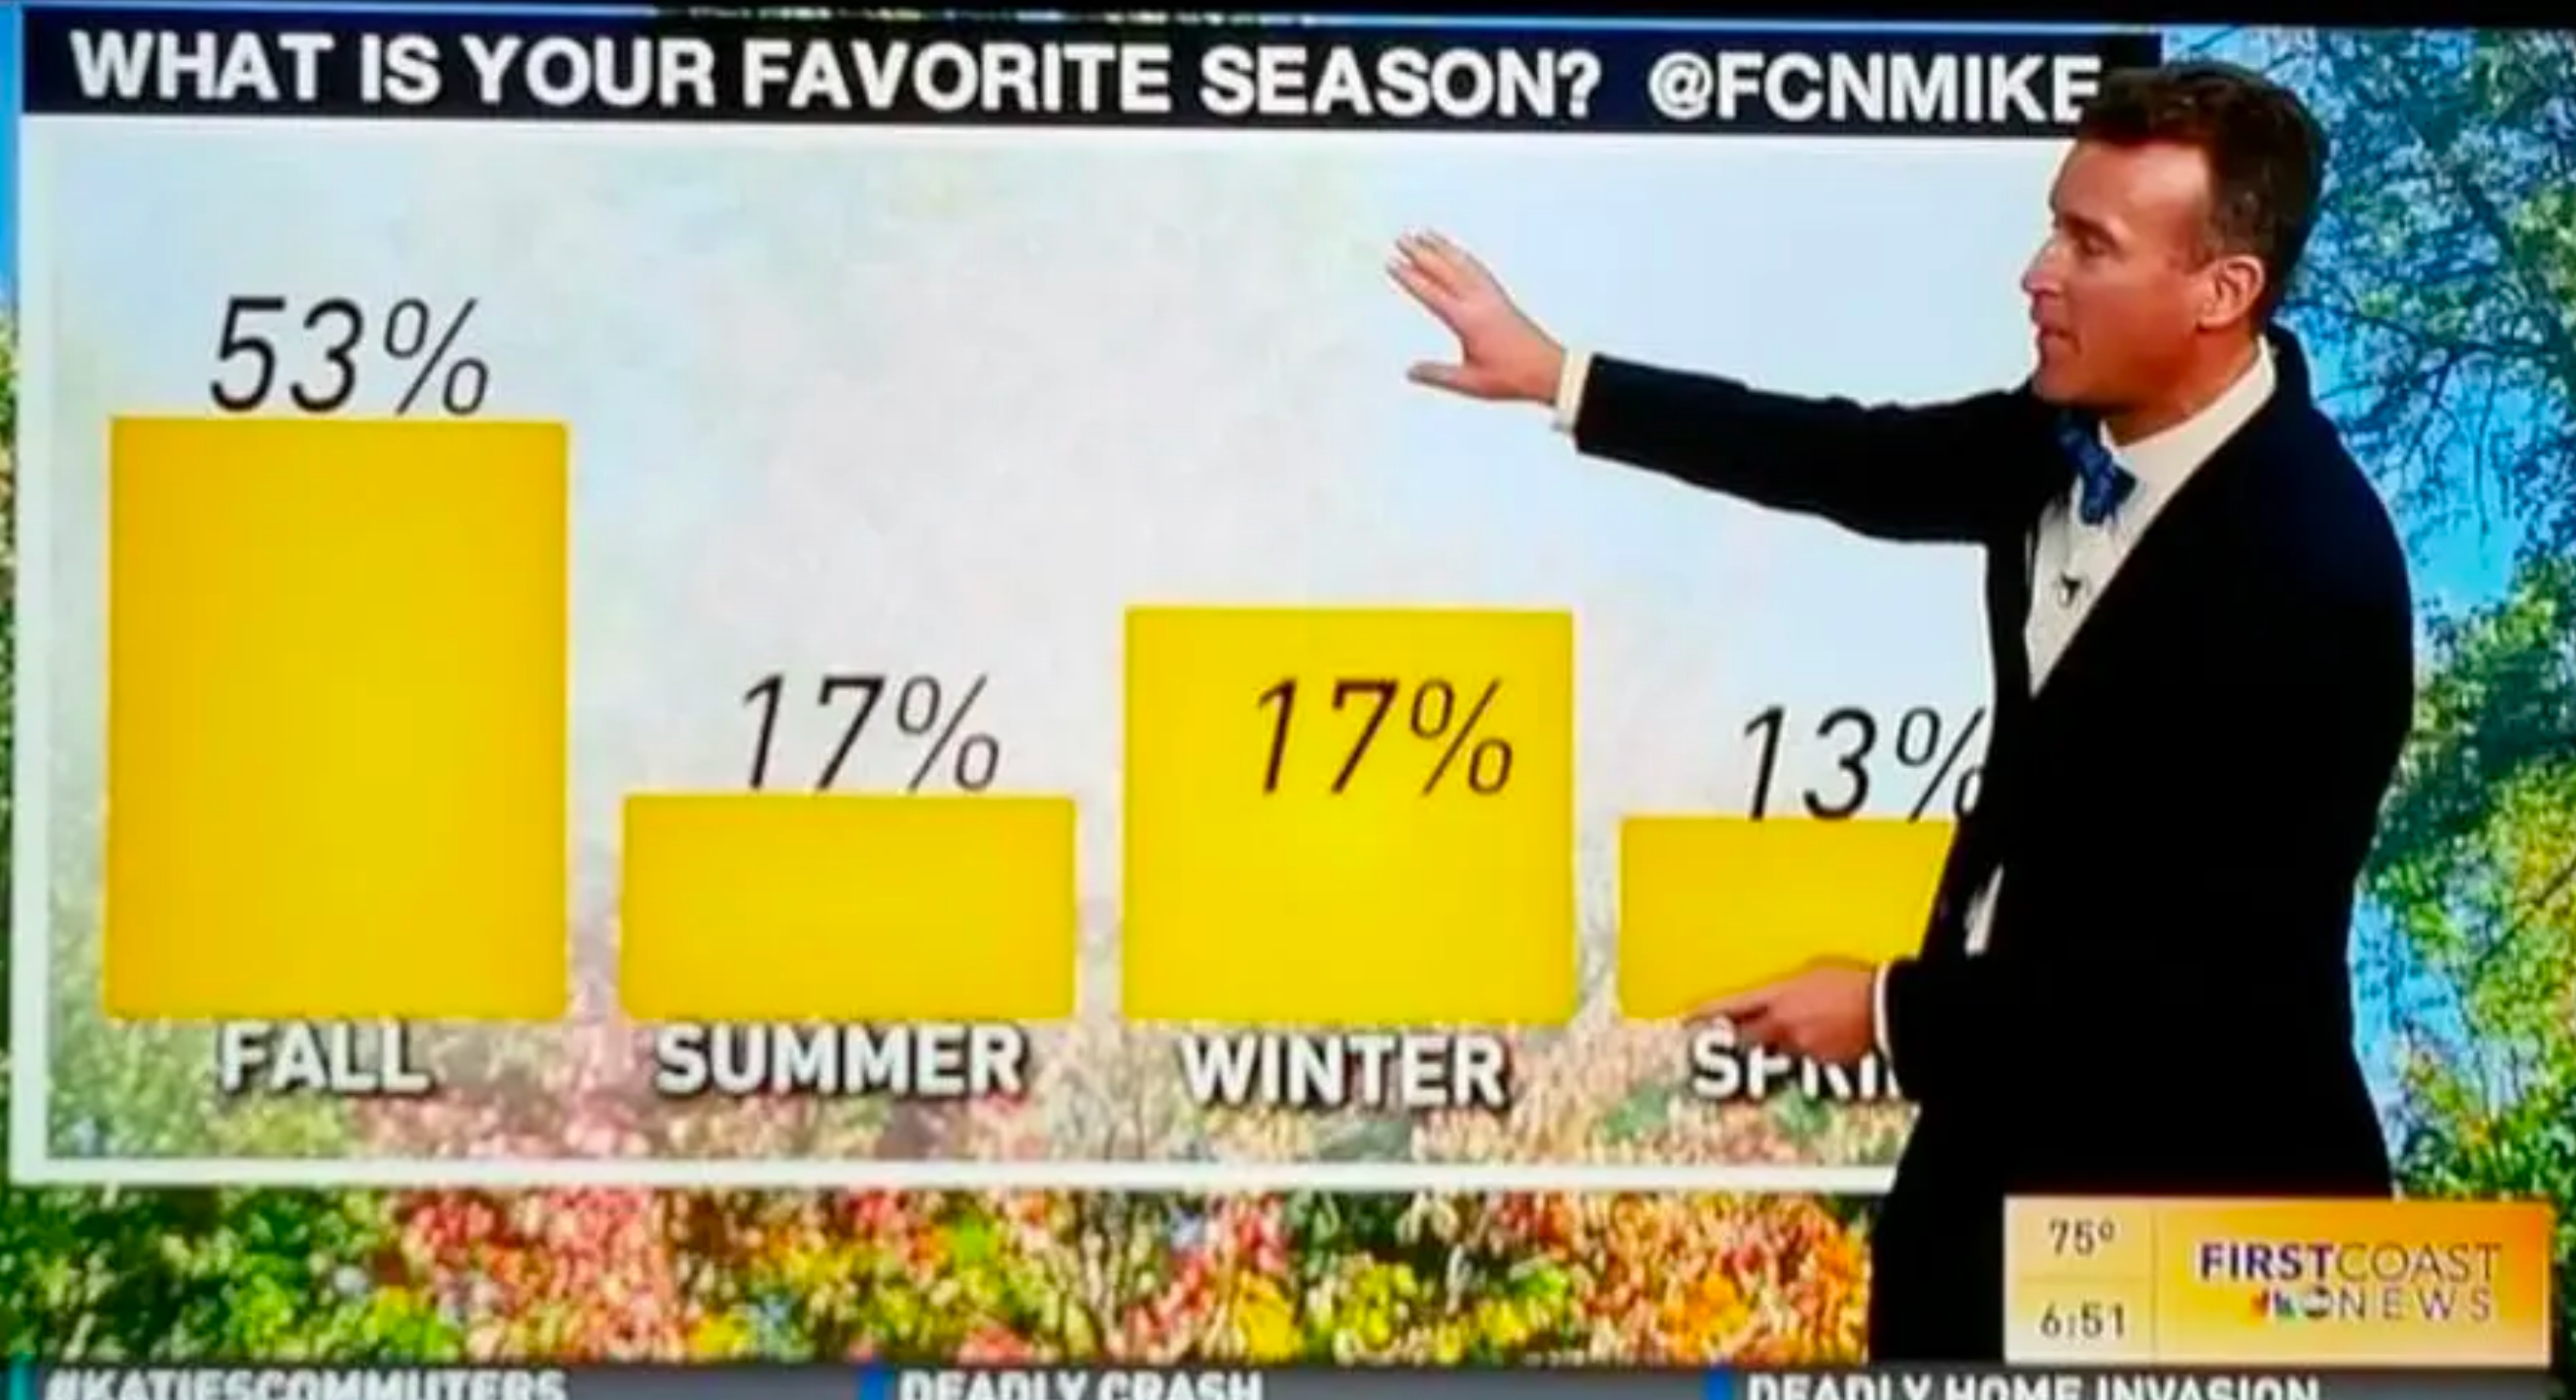
\includegraphics[keepaspectratio]{hallofshame_figs/fig_19.png}}
\end{frame}

\begin{frame}{Plotting pitfalls}
\phantomsection\label{plotting-pitfalls-2}
\begin{itemize}
\tightlist
\item
  Axis trickery (a.k.a. ``little y lies'')
\item
  Violations of basic math
\item
  \textcolor{orange}{Nearly content-free figures}
\item
  Gratuitous chartjunk
\item
  Poorly chosen 3D graphics
\item
  Bad design choices
\end{itemize}
\end{frame}

\begin{frame}{}
\phantomsection\label{section-13}
\pandocbounded{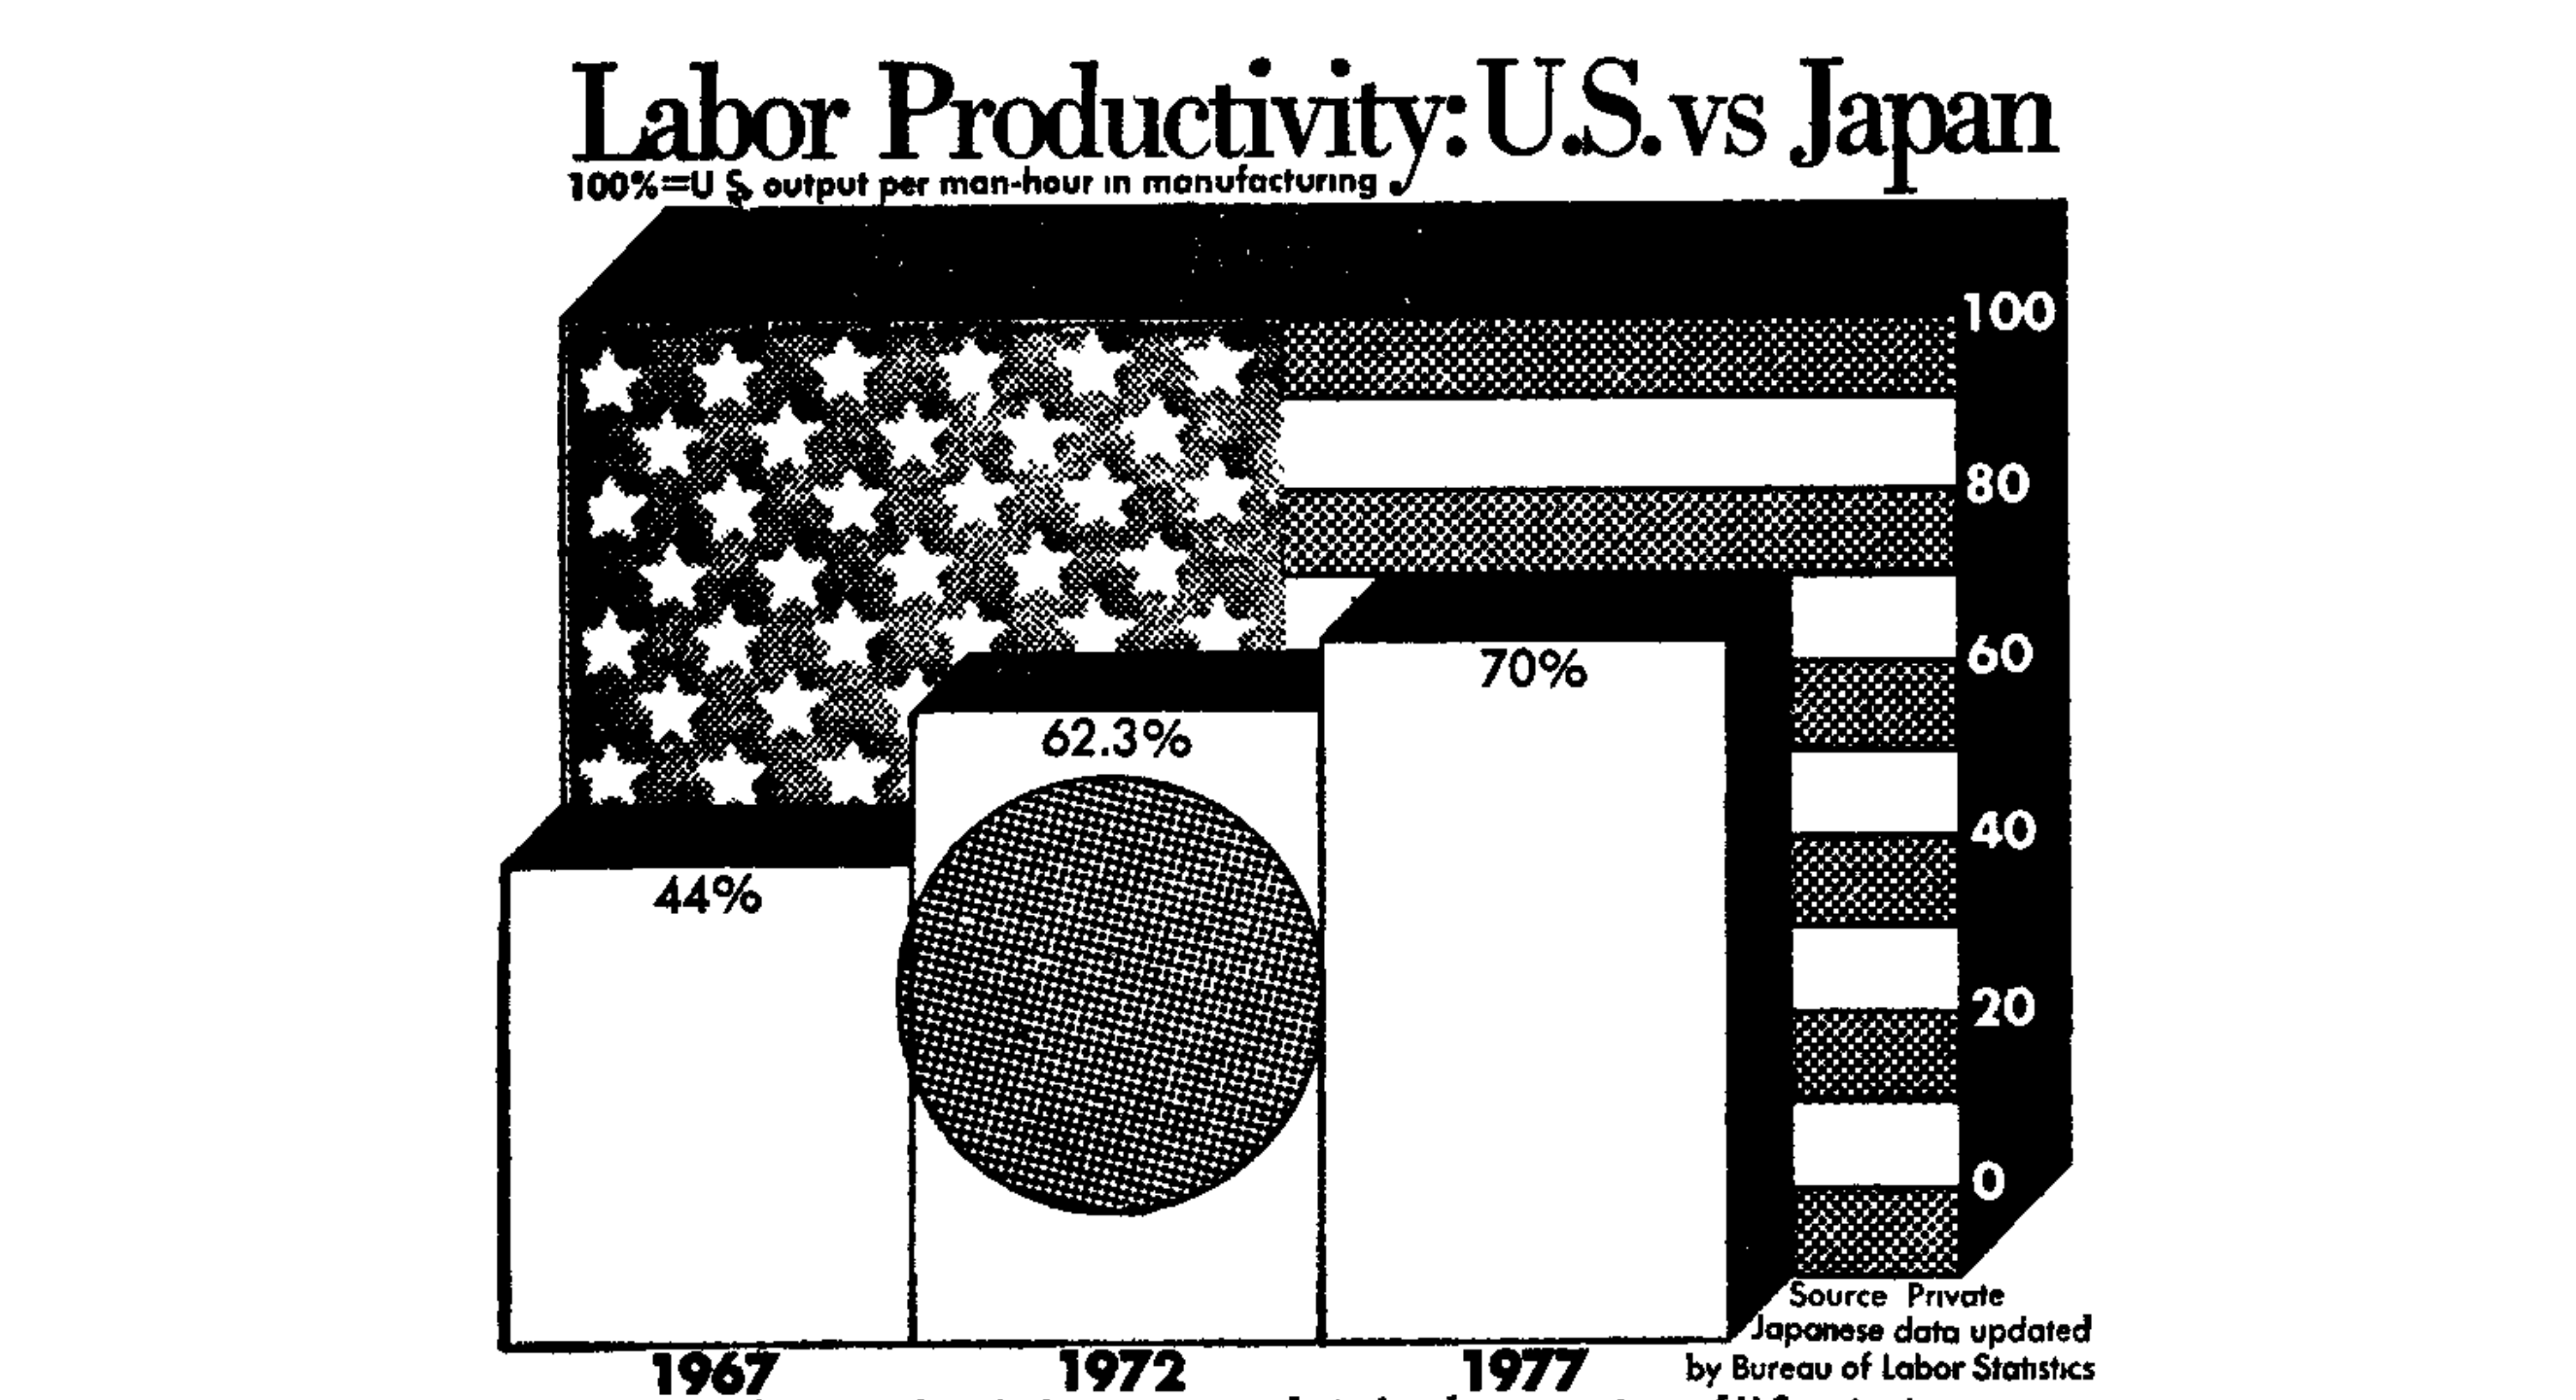
\includegraphics[keepaspectratio]{hallofshame_figs/fig_21.png}}
\end{frame}

\begin{frame}{}
\phantomsection\label{section-14}
\pandocbounded{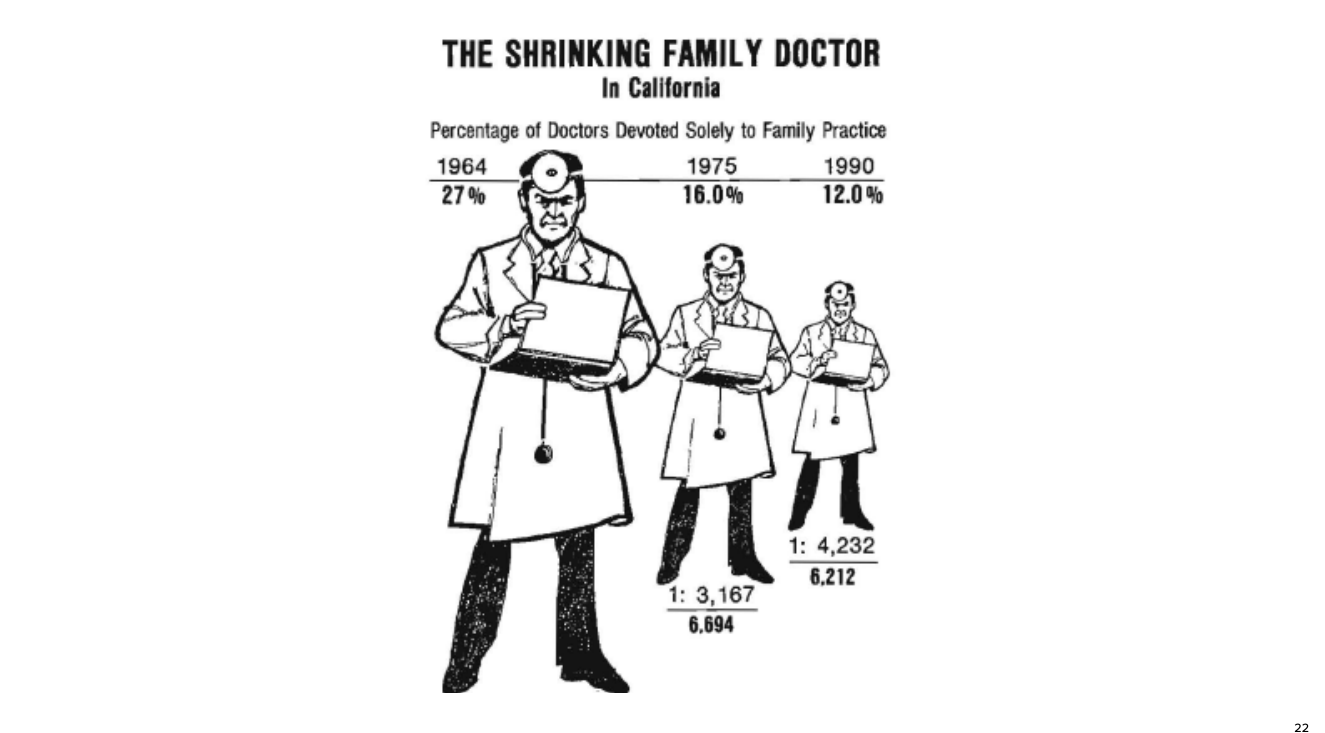
\includegraphics[keepaspectratio]{hallofshame_figs/fig_22.png}}
\end{frame}

\begin{frame}{}
\phantomsection\label{section-15}
\pandocbounded{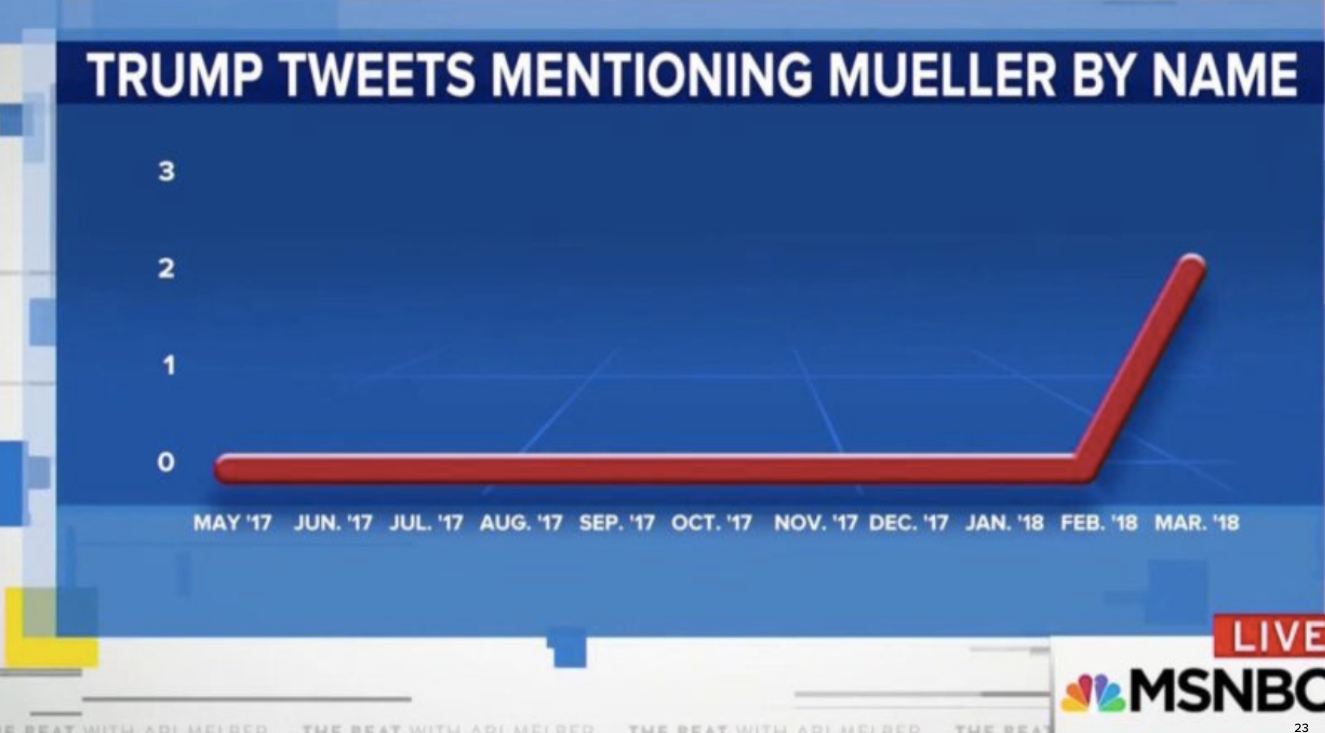
\includegraphics[keepaspectratio]{hallofshame_figs/fig_23.png}}
\end{frame}

\begin{frame}{Plotting pitfalls}
\phantomsection\label{plotting-pitfalls-3}
\begin{itemize}
\tightlist
\item
  Axis trickery (a.k.a. ``little y lies'')
\item
  Violations of basic math
\item
  Nearly content-free figures
\item
  \textcolor{orange}{Gratuitous chartjunk}
\item
  Poorly chosen 3D graphics
\item
  Bad design choices
\end{itemize}
\end{frame}

\begin{frame}{}
\phantomsection\label{section-16}
\pandocbounded{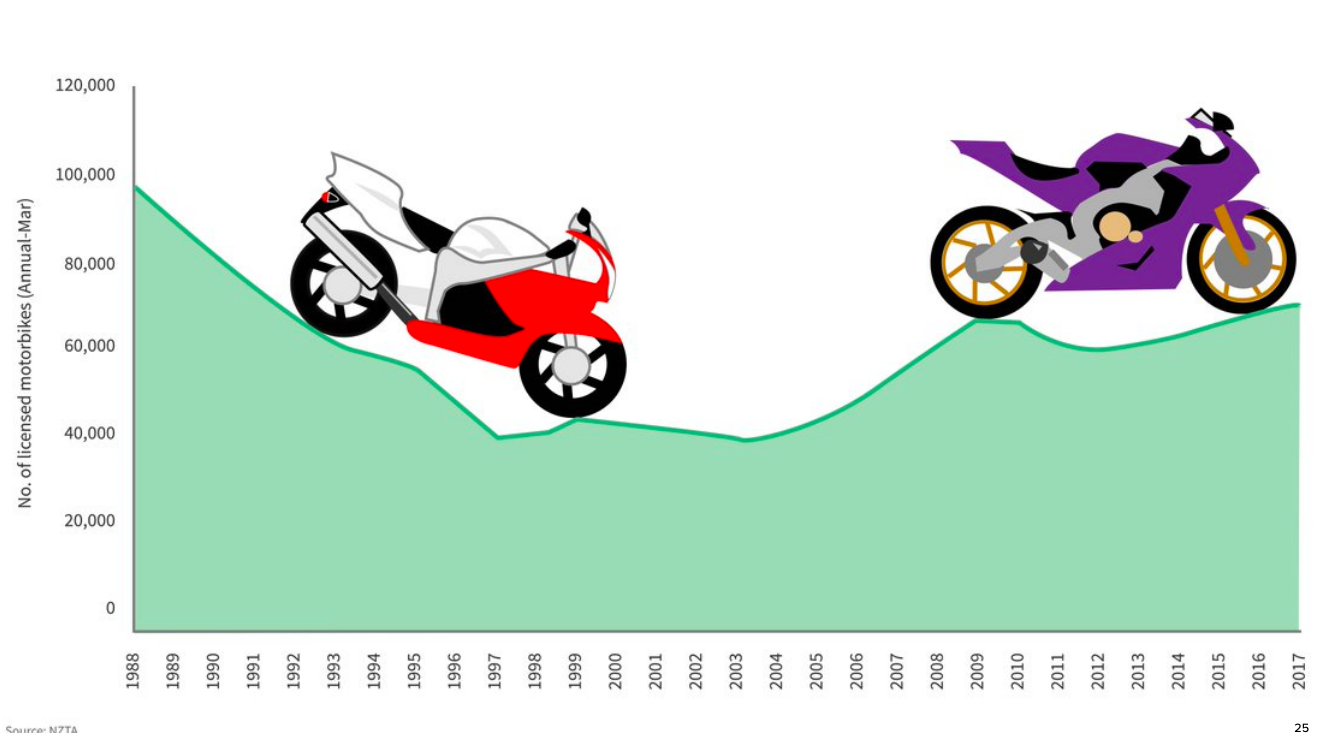
\includegraphics[keepaspectratio]{hallofshame_figs/fig_25.png}}
\end{frame}

\begin{frame}{}
\phantomsection\label{section-17}
\pandocbounded{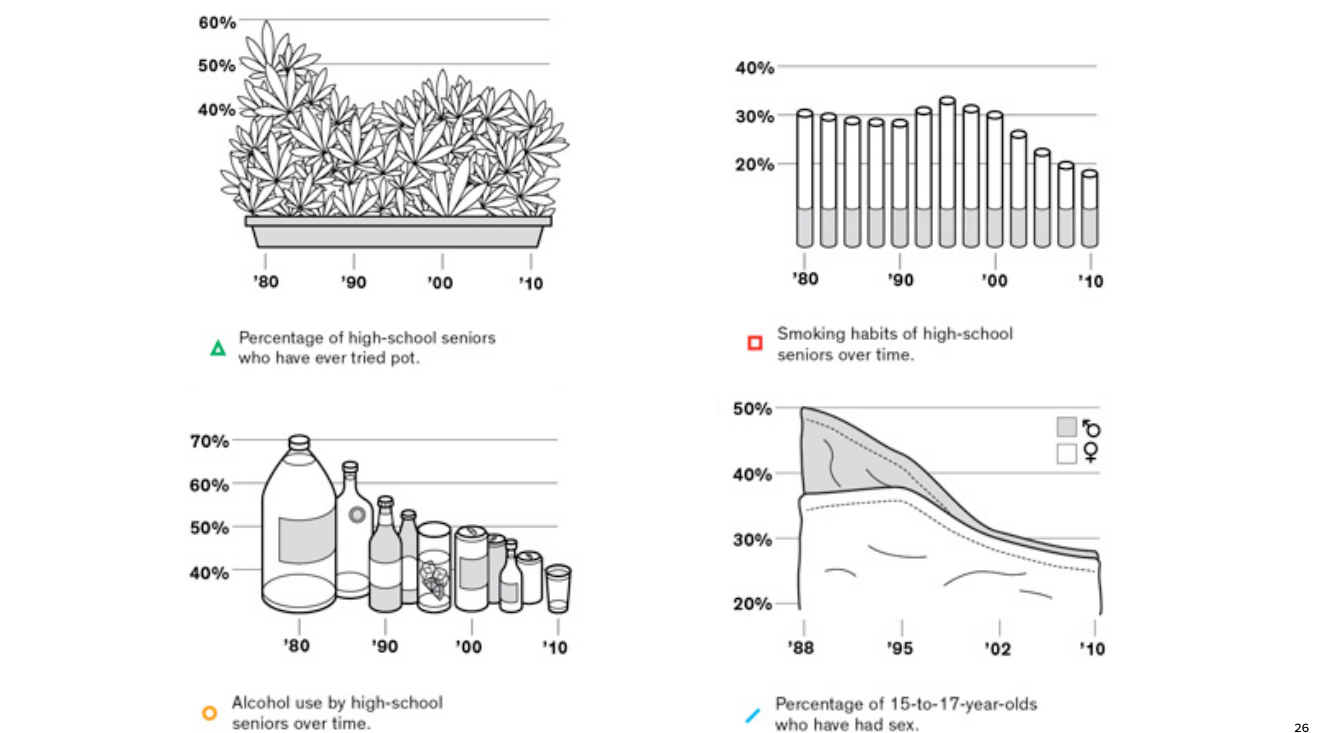
\includegraphics[keepaspectratio]{hallofshame_figs/fig_26.png}}
\end{frame}

\begin{frame}{}
\phantomsection\label{section-18}
\pandocbounded{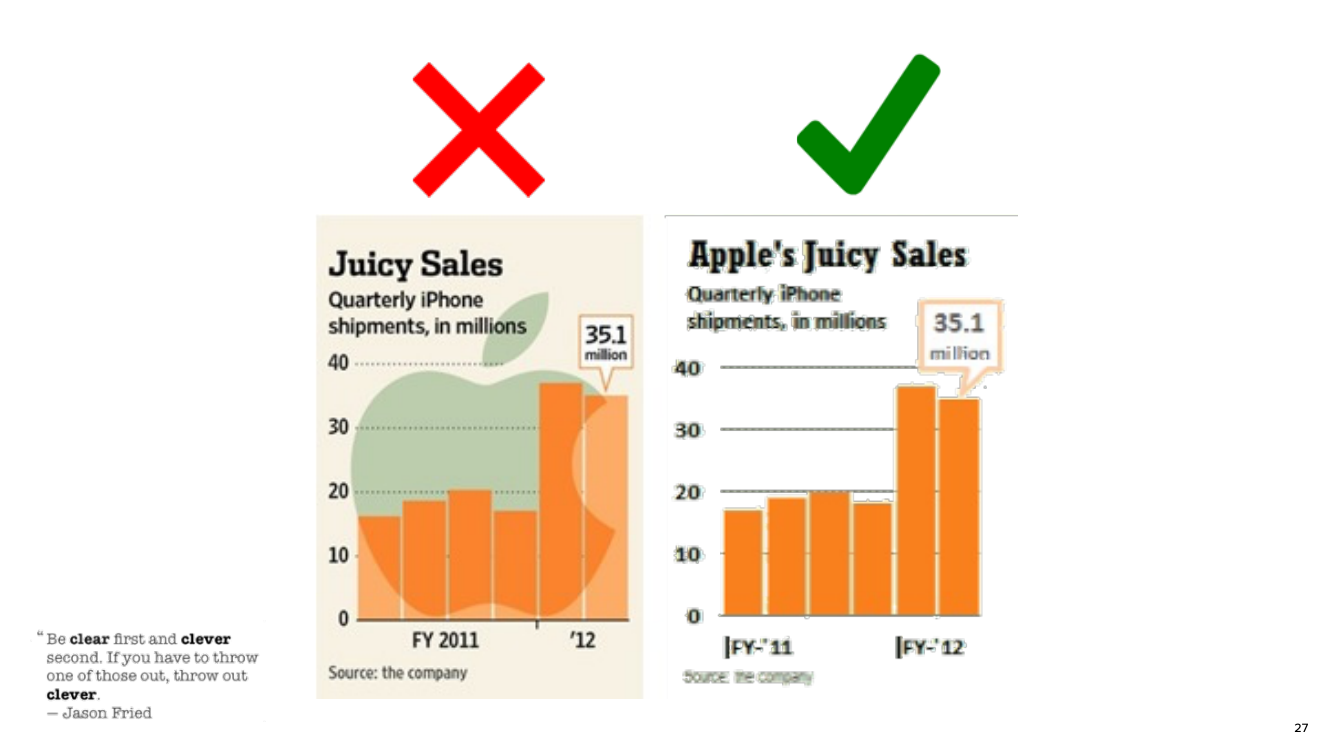
\includegraphics[keepaspectratio]{hallofshame_figs/fig_27.png}}
\end{frame}

\begin{frame}{Plotting pitfalls}
\phantomsection\label{plotting-pitfalls-4}
\begin{itemize}
\tightlist
\item
  Axis trickery (a.k.a. ``little y lies'')
\item
  Violations of basic math
\item
  Nearly content-free figures
\item
  Gratuitous chartjunk
\item
  \textcolor{orange}{Poorly chosen 3D graphics}
\item
  Bad design choices
\end{itemize}
\end{frame}

\begin{frame}{}
\phantomsection\label{section-19}
\pandocbounded{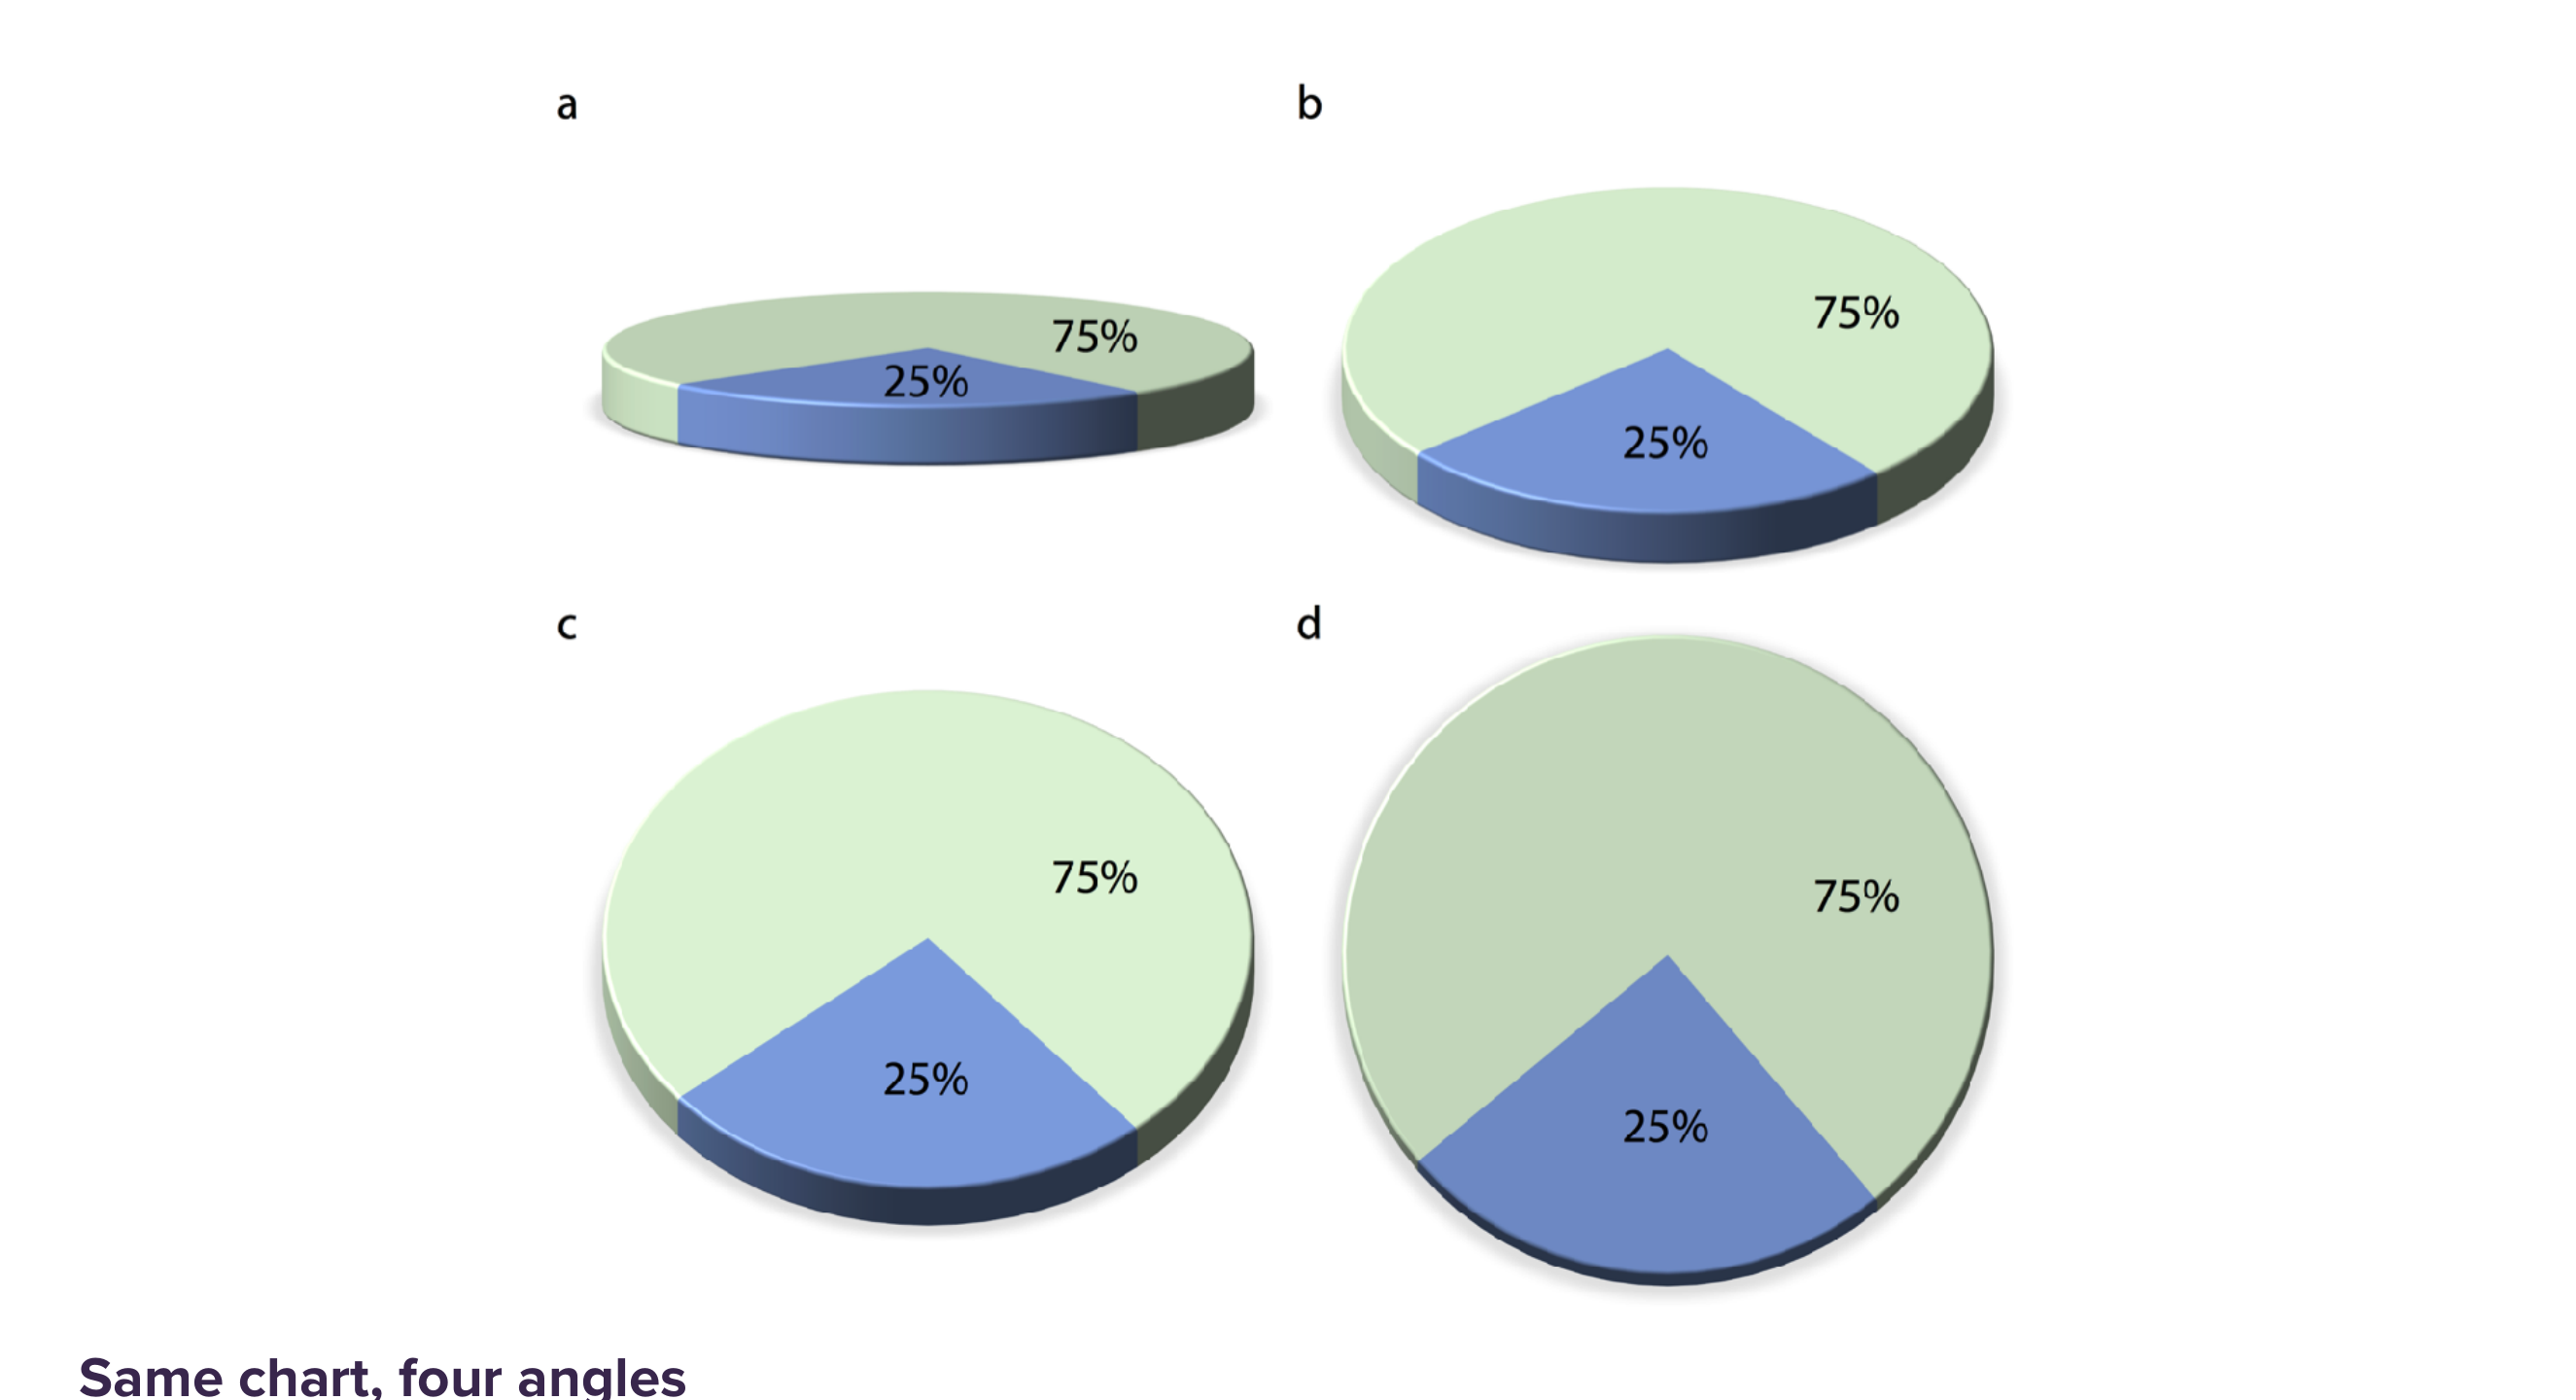
\includegraphics[keepaspectratio]{hallofshame_figs/fig_29.png}}
\end{frame}

\begin{frame}{}
\phantomsection\label{section-20}
\pandocbounded{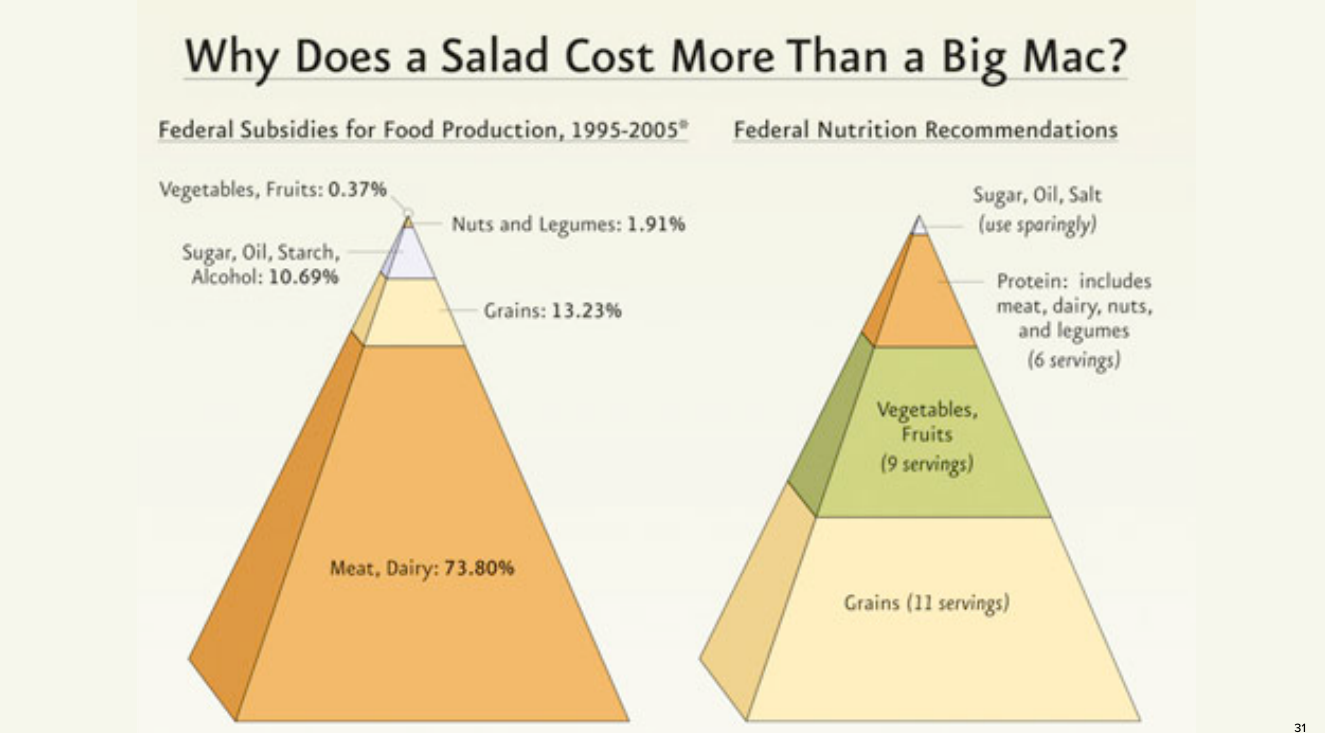
\includegraphics[keepaspectratio]{hallofshame_figs/fig_30.png}}
\end{frame}

\begin{frame}{}
\phantomsection\label{section-21}
\pandocbounded{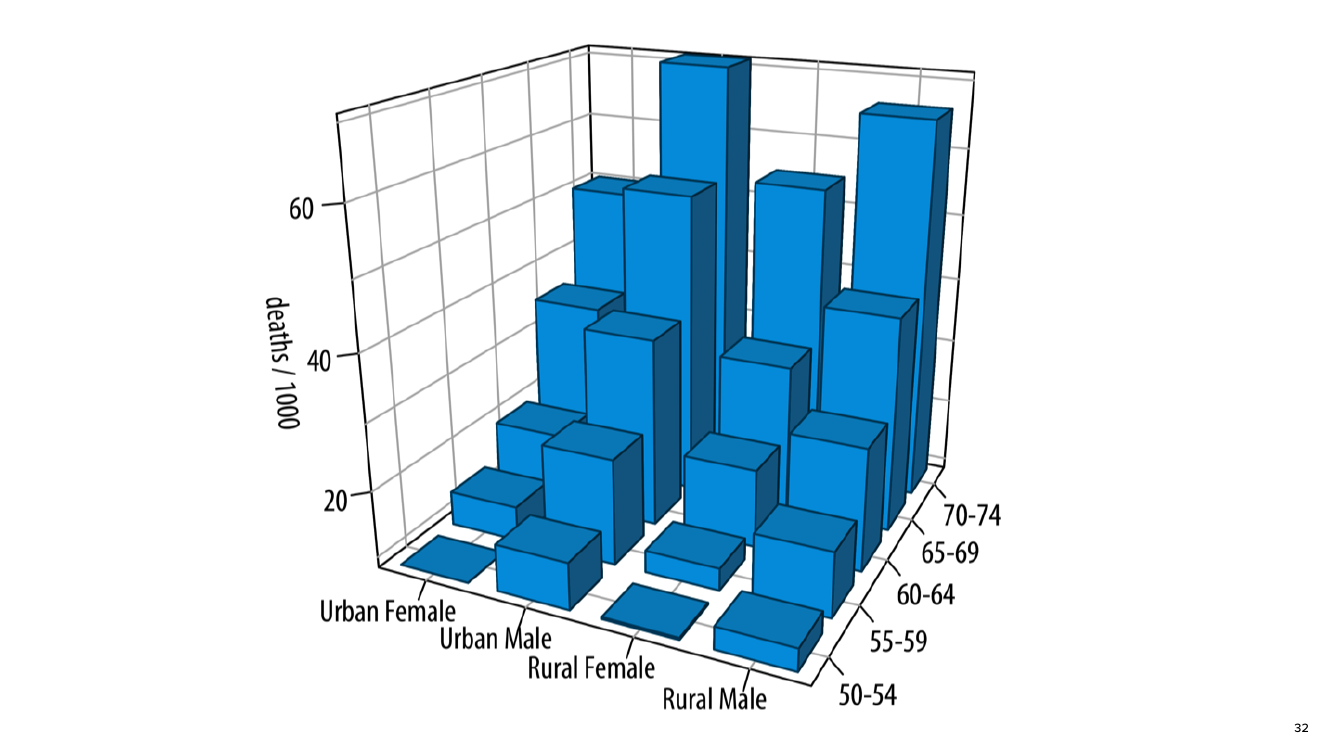
\includegraphics[keepaspectratio]{hallofshame_figs/fig_31.png}}
\end{frame}

\begin{frame}{}
\phantomsection\label{section-22}
\pandocbounded{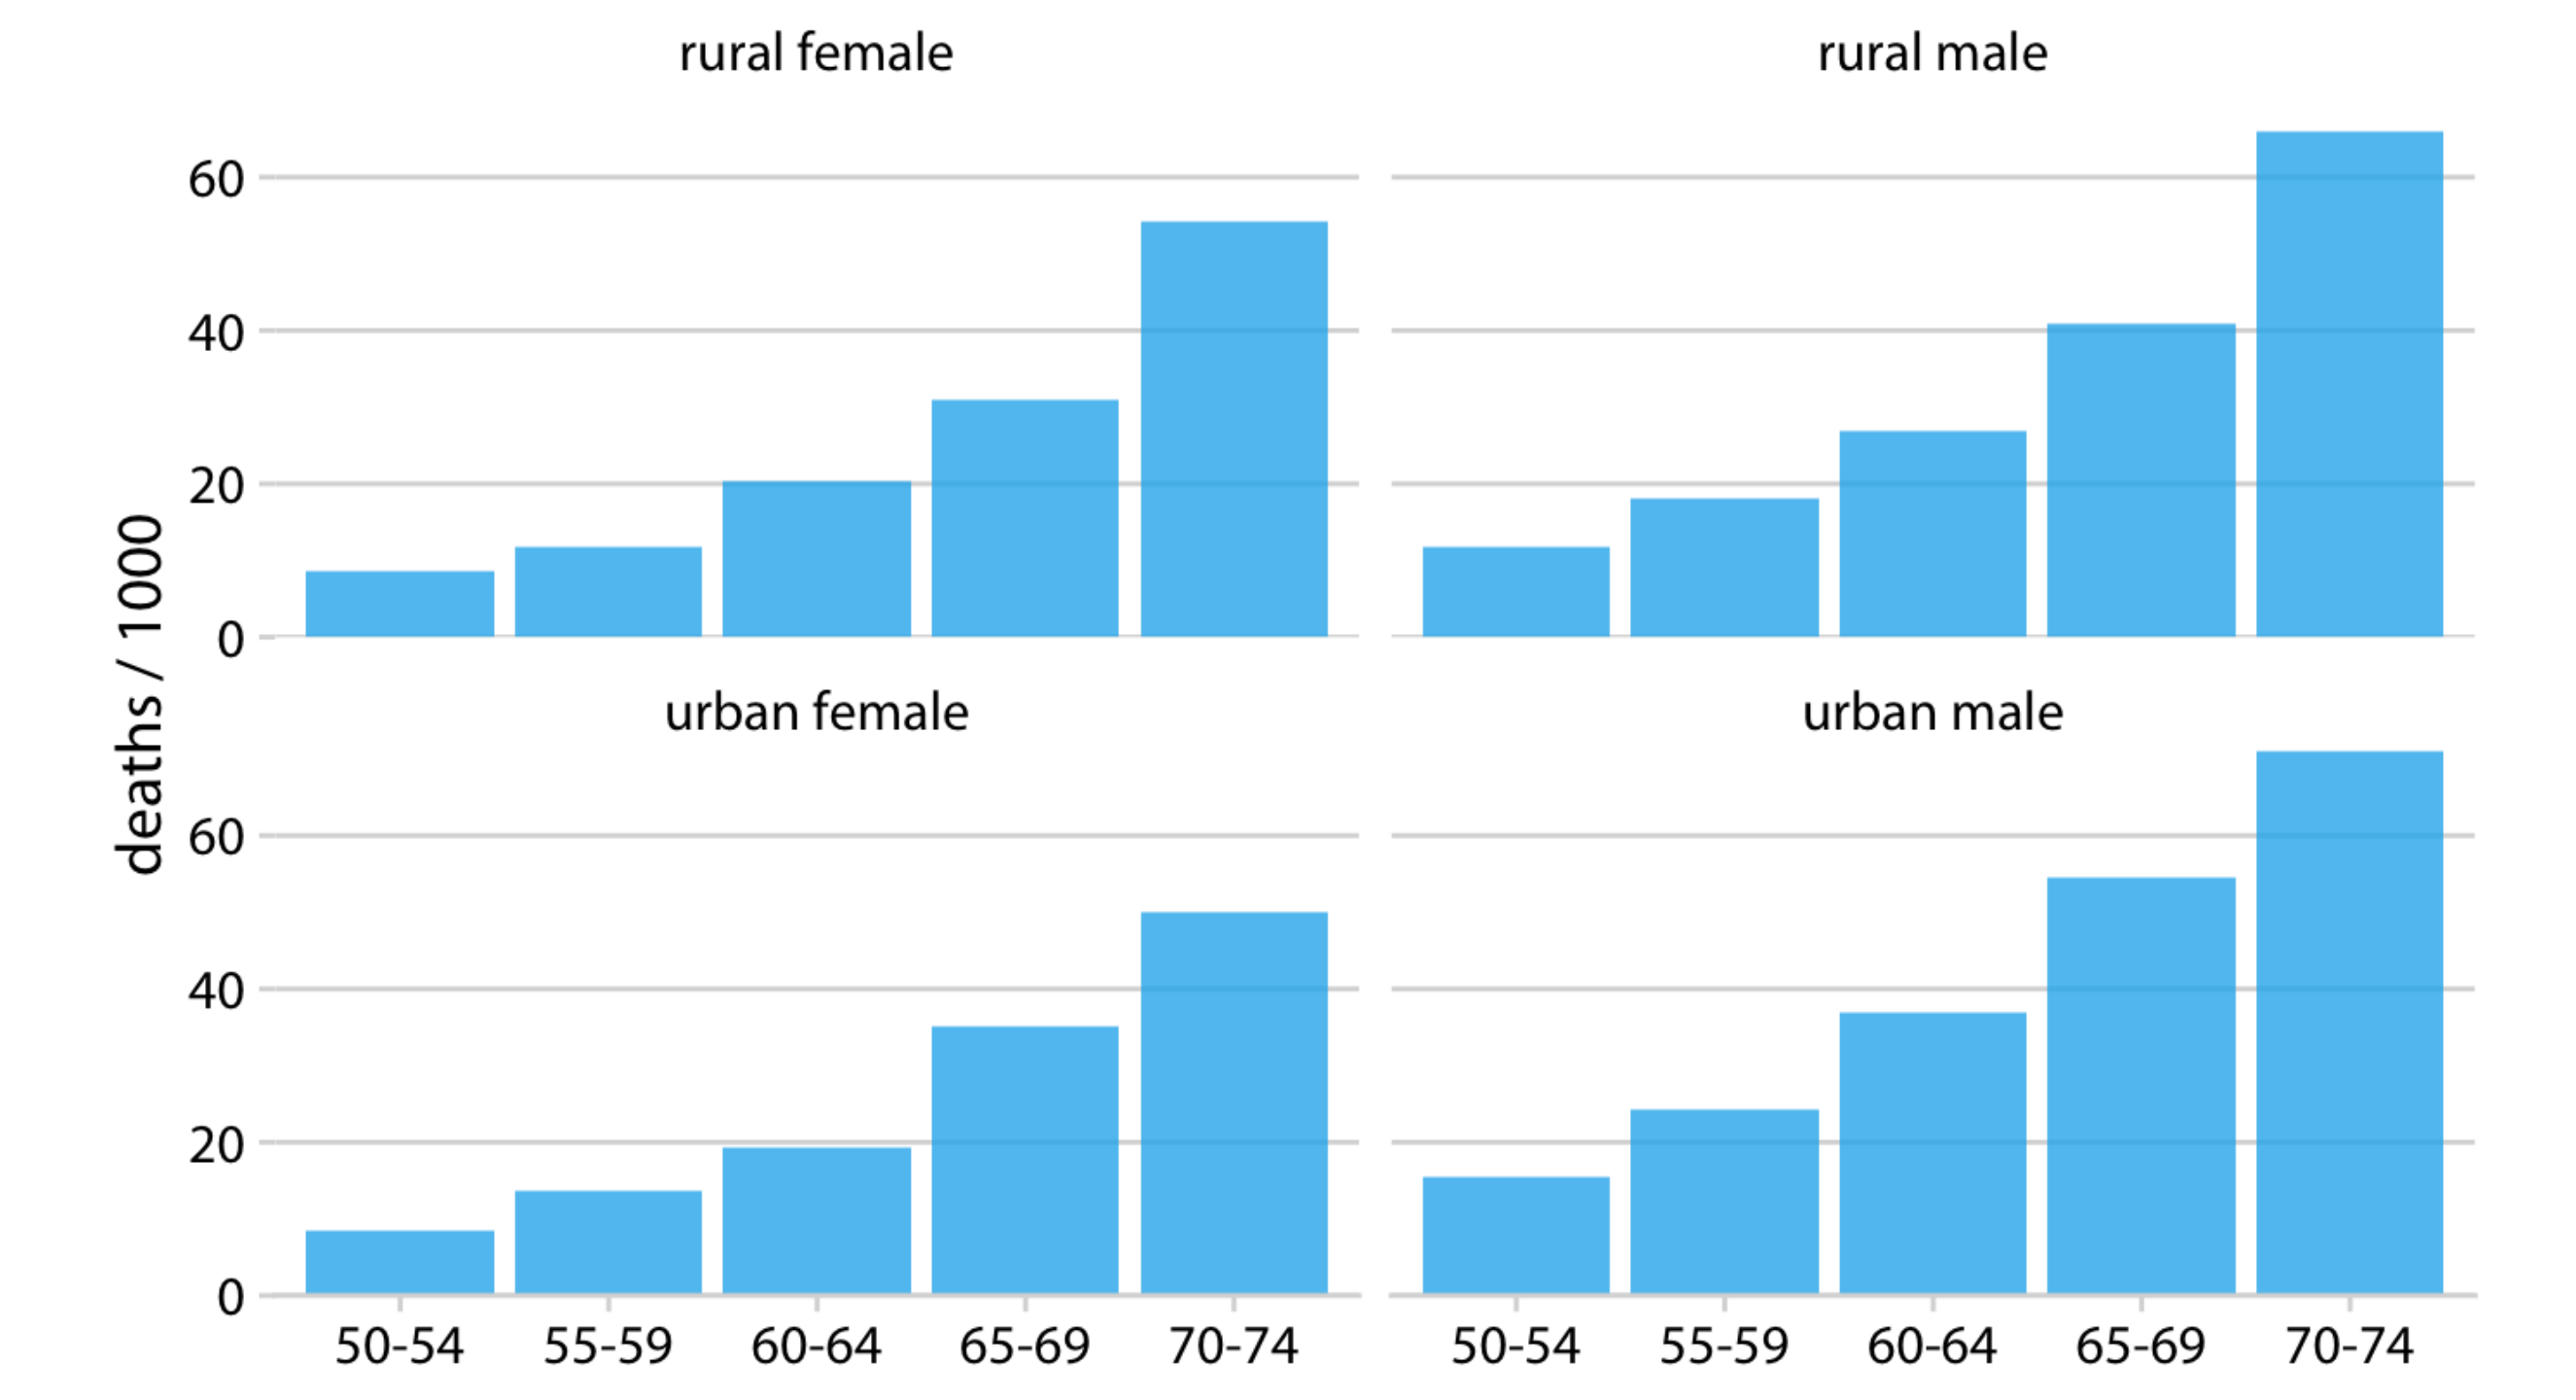
\includegraphics[keepaspectratio]{hallofshame_figs/fig_32.png}}
\end{frame}

\begin{frame}{Plotting pitfalls}
\phantomsection\label{plotting-pitfalls-5}
\begin{itemize}
\tightlist
\item
  Axis trickery (a.k.a. ``little y lies'')
\item
  Violations of basic math
\item
  Nearly content-free figures
\item
  Gratuitous chartjunk
\item
  Poorly chosen 3D graphics
\item
  \textcolor{orange}{Bad design choices}
\end{itemize}
\end{frame}

\begin{frame}{}
\phantomsection\label{section-23}
\pandocbounded{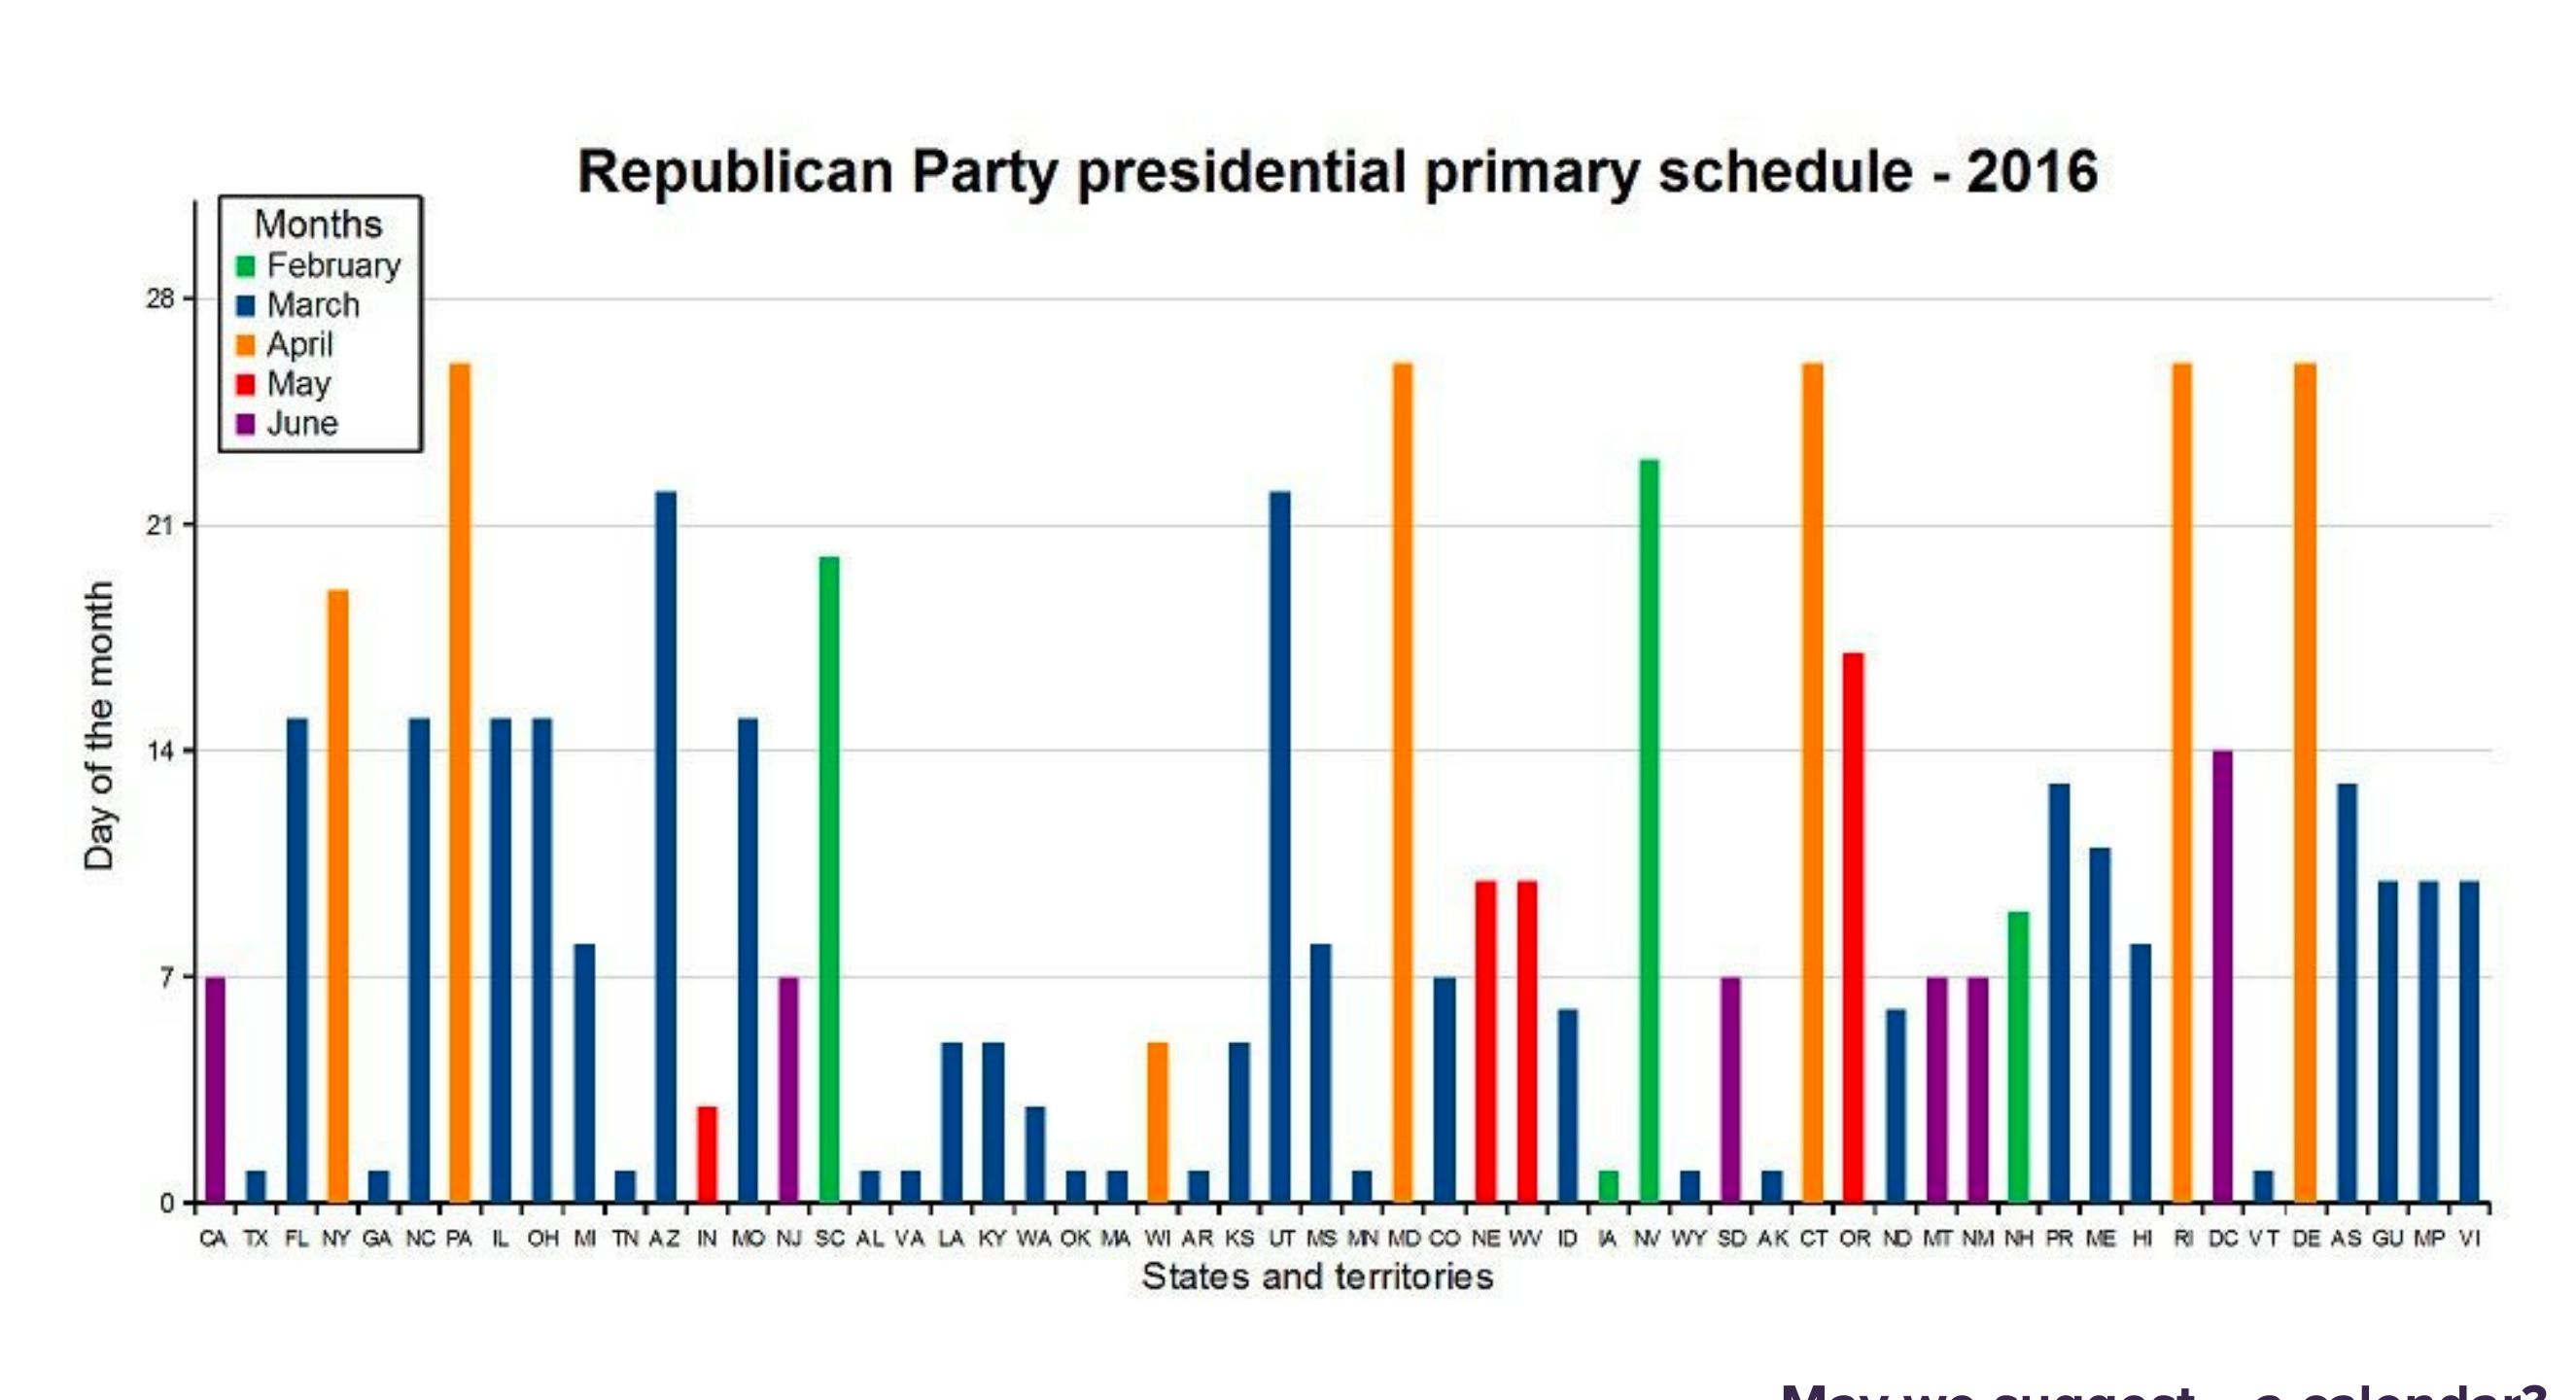
\includegraphics[keepaspectratio]{hallofshame_figs/fig_34.png}}
\end{frame}

\begin{frame}{}
\phantomsection\label{section-24}
\pandocbounded{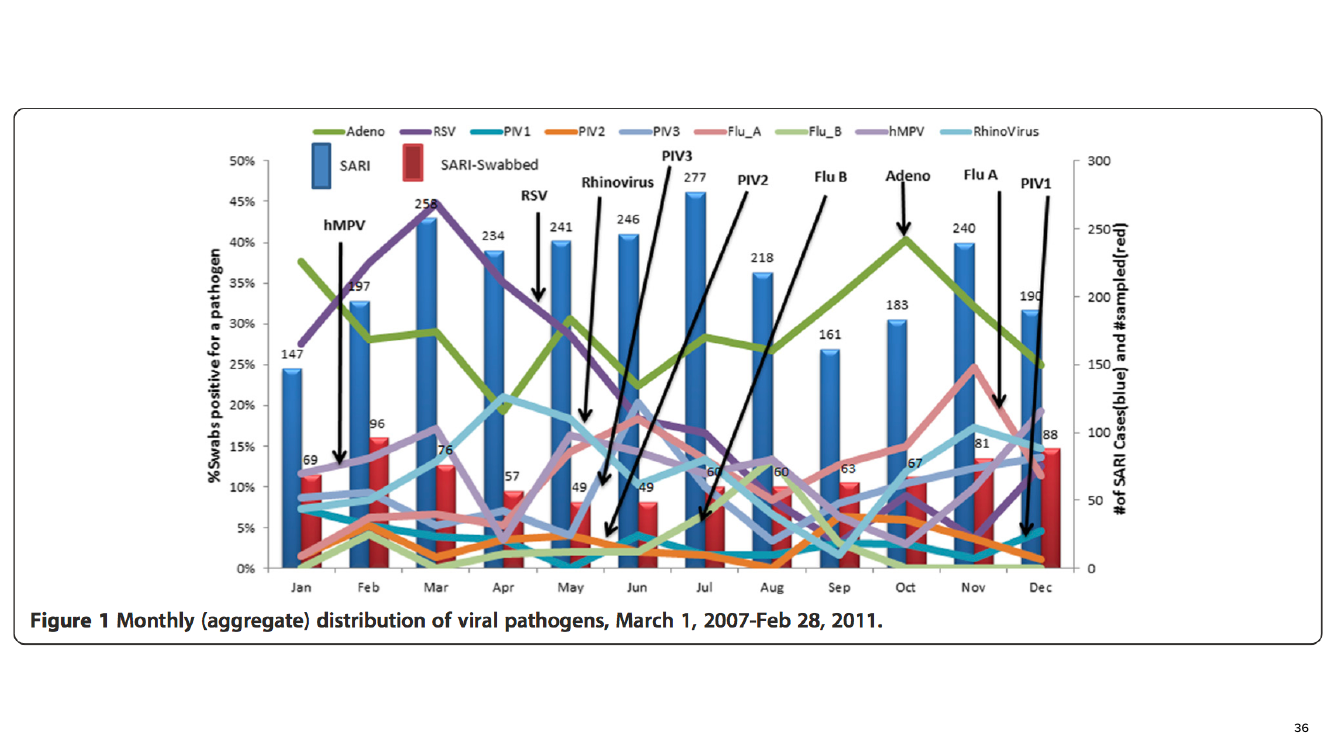
\includegraphics[keepaspectratio]{hallofshame_figs/fig_35.png}}
\end{frame}

\begin{frame}{}
\phantomsection\label{section-25}
\pandocbounded{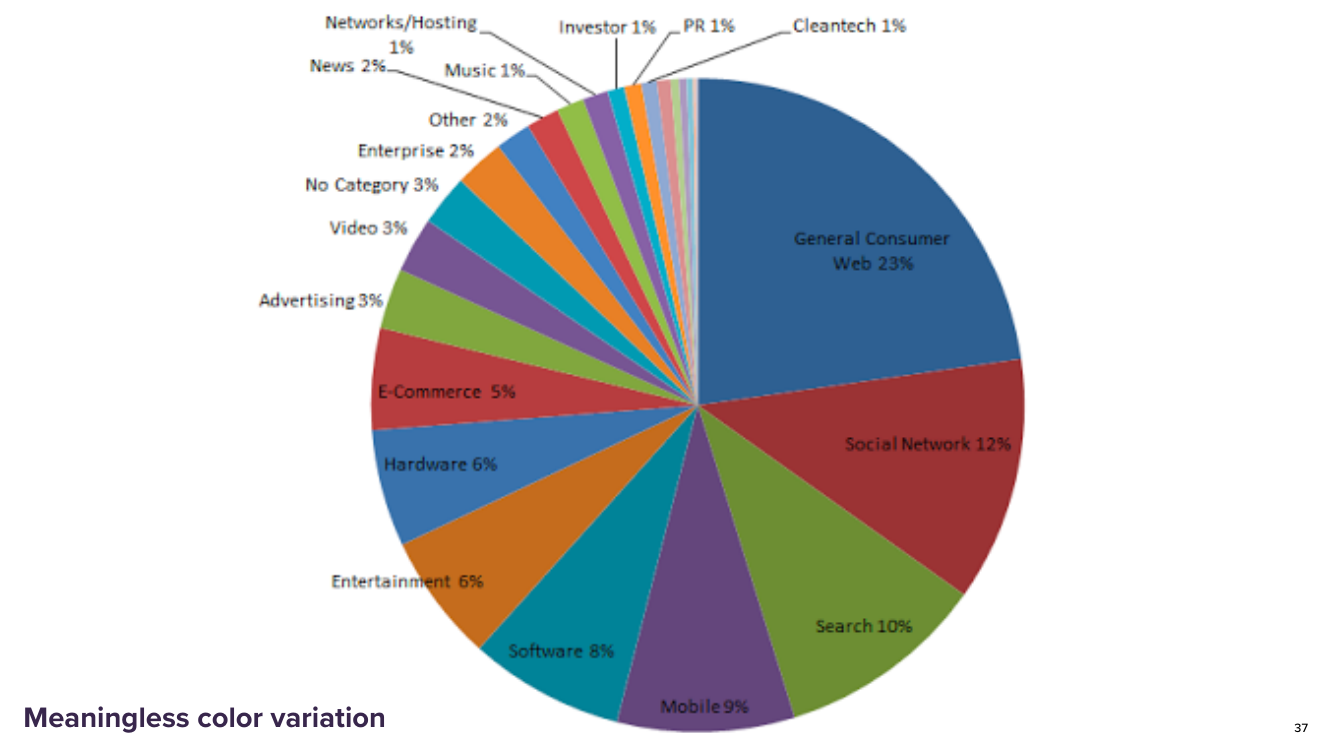
\includegraphics[keepaspectratio]{hallofshame_figs/fig_36.png}}
\end{frame}

\begin{frame}{}
\phantomsection\label{section-26}
\pandocbounded{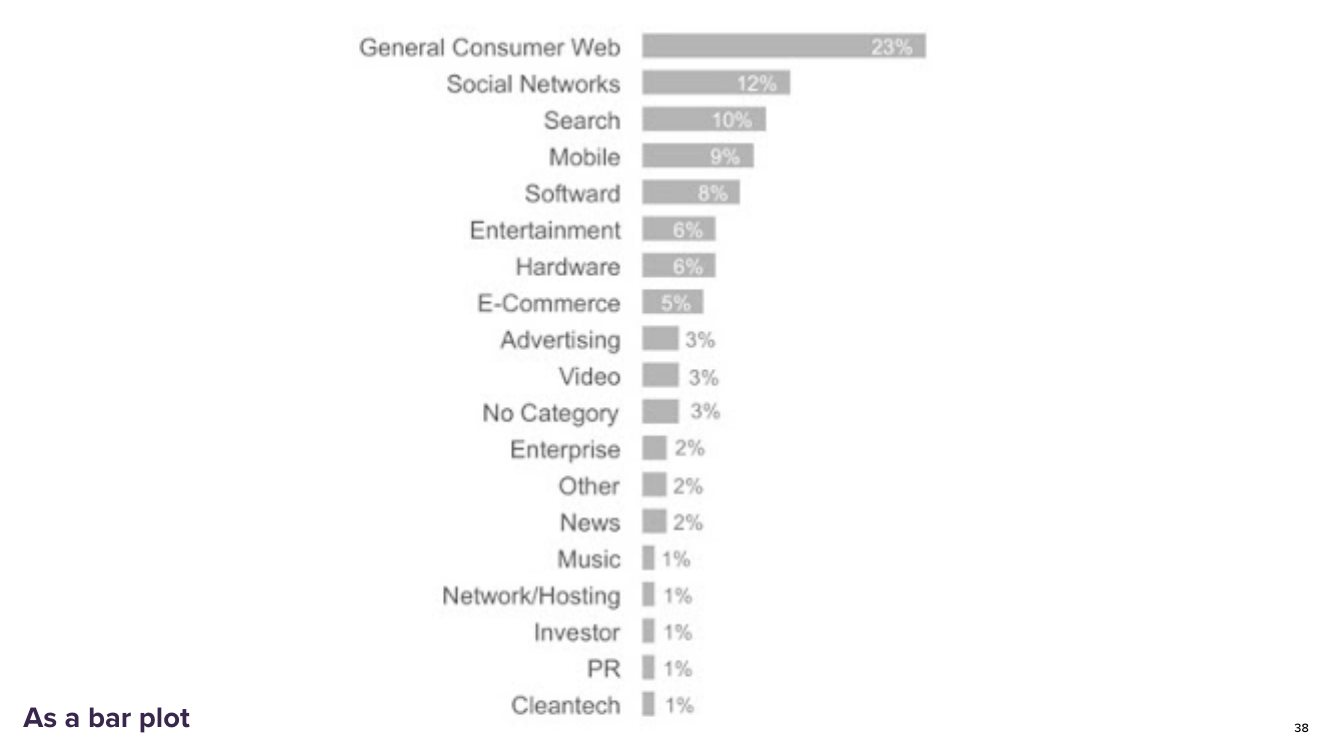
\includegraphics[keepaspectratio]{hallofshame_figs/fig_37.png}}
\end{frame}

\begin{frame}{}
\phantomsection\label{section-27}
\pandocbounded{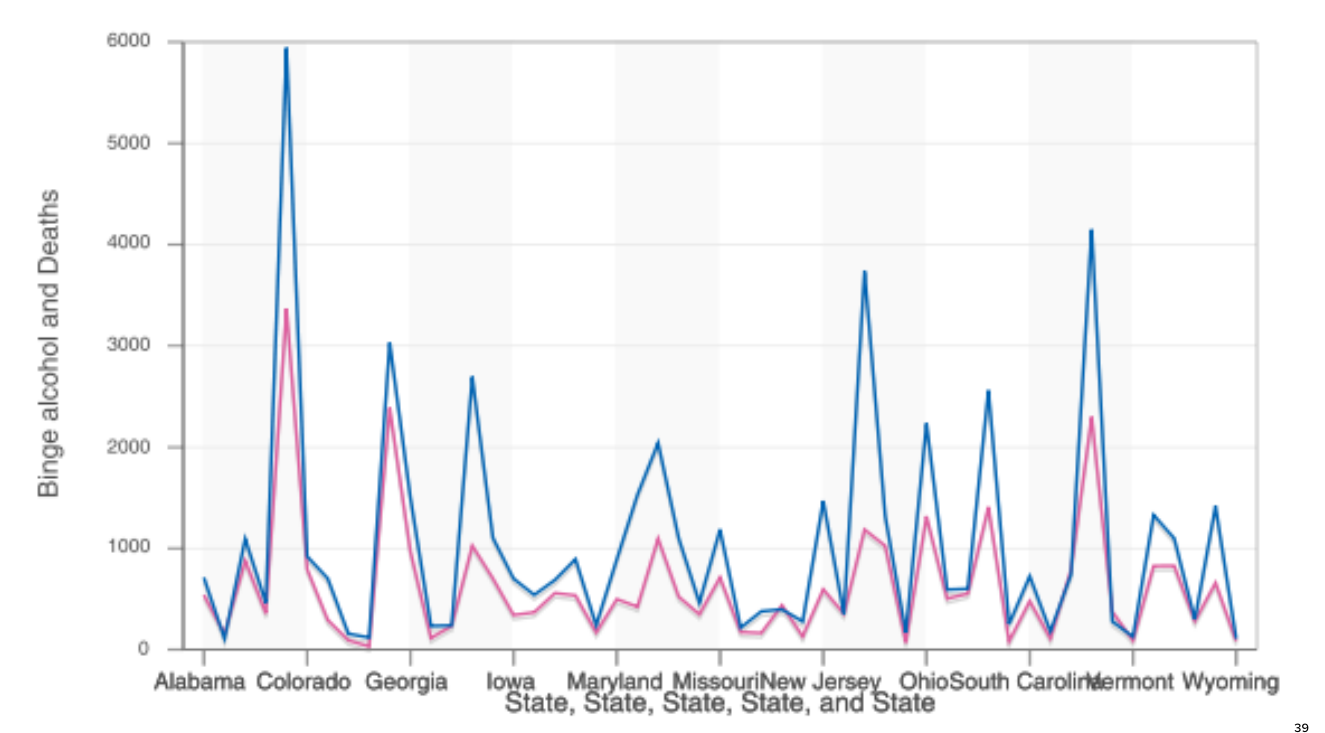
\includegraphics[keepaspectratio]{hallofshame_figs/fig_38.png}}
\end{frame}

\begin{frame}{}
\phantomsection\label{section-28}
\pandocbounded{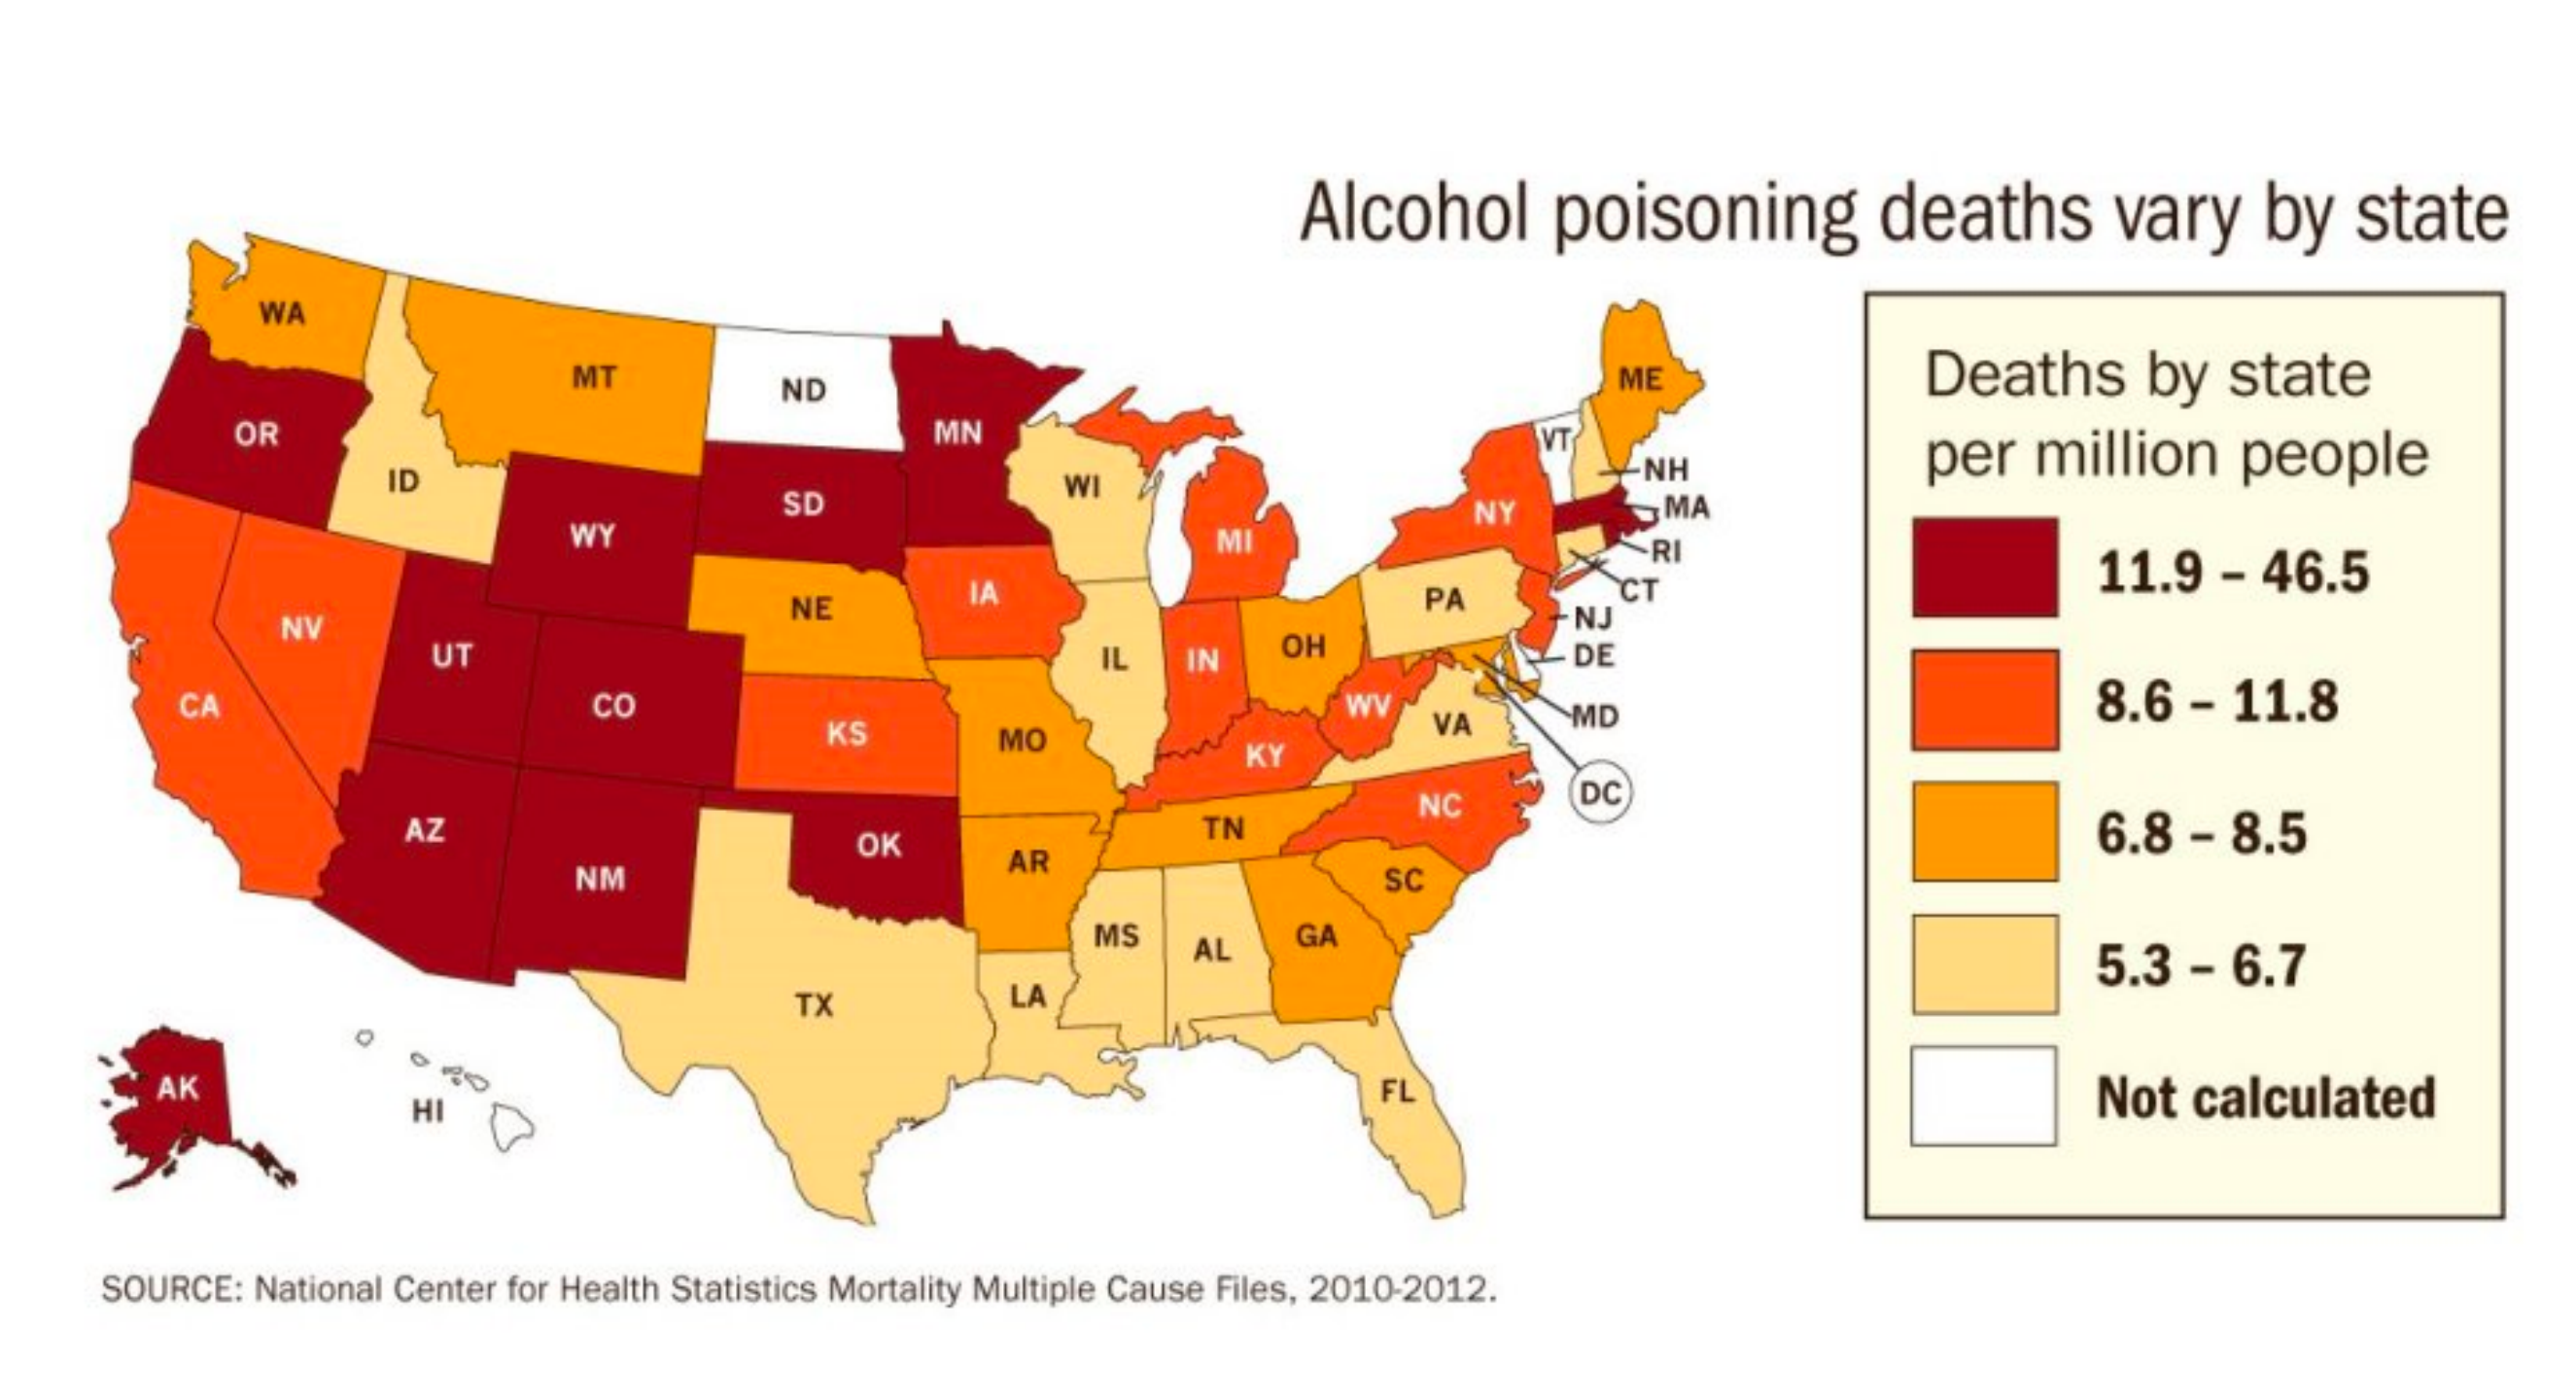
\includegraphics[keepaspectratio]{hallofshame_figs/fig_39.png}}
\end{frame}

\begin{frame}{Your turn!}
\phantomsection\label{your-turn}
\begin{itemize}
\tightlist
\item
  Break in the groups of 2-3 and answer the following questions about
  the next figure:
\end{itemize}

\begin{enumerate}
  \item What is this figure trying to convey, and is it successful or not?
  \item If successful, what features make it so?  If unsuccessful, what would you change to make it the best graphic ever?
\end{enumerate}
\end{frame}

\begin{frame}{}
\phantomsection\label{section-29}
\pandocbounded{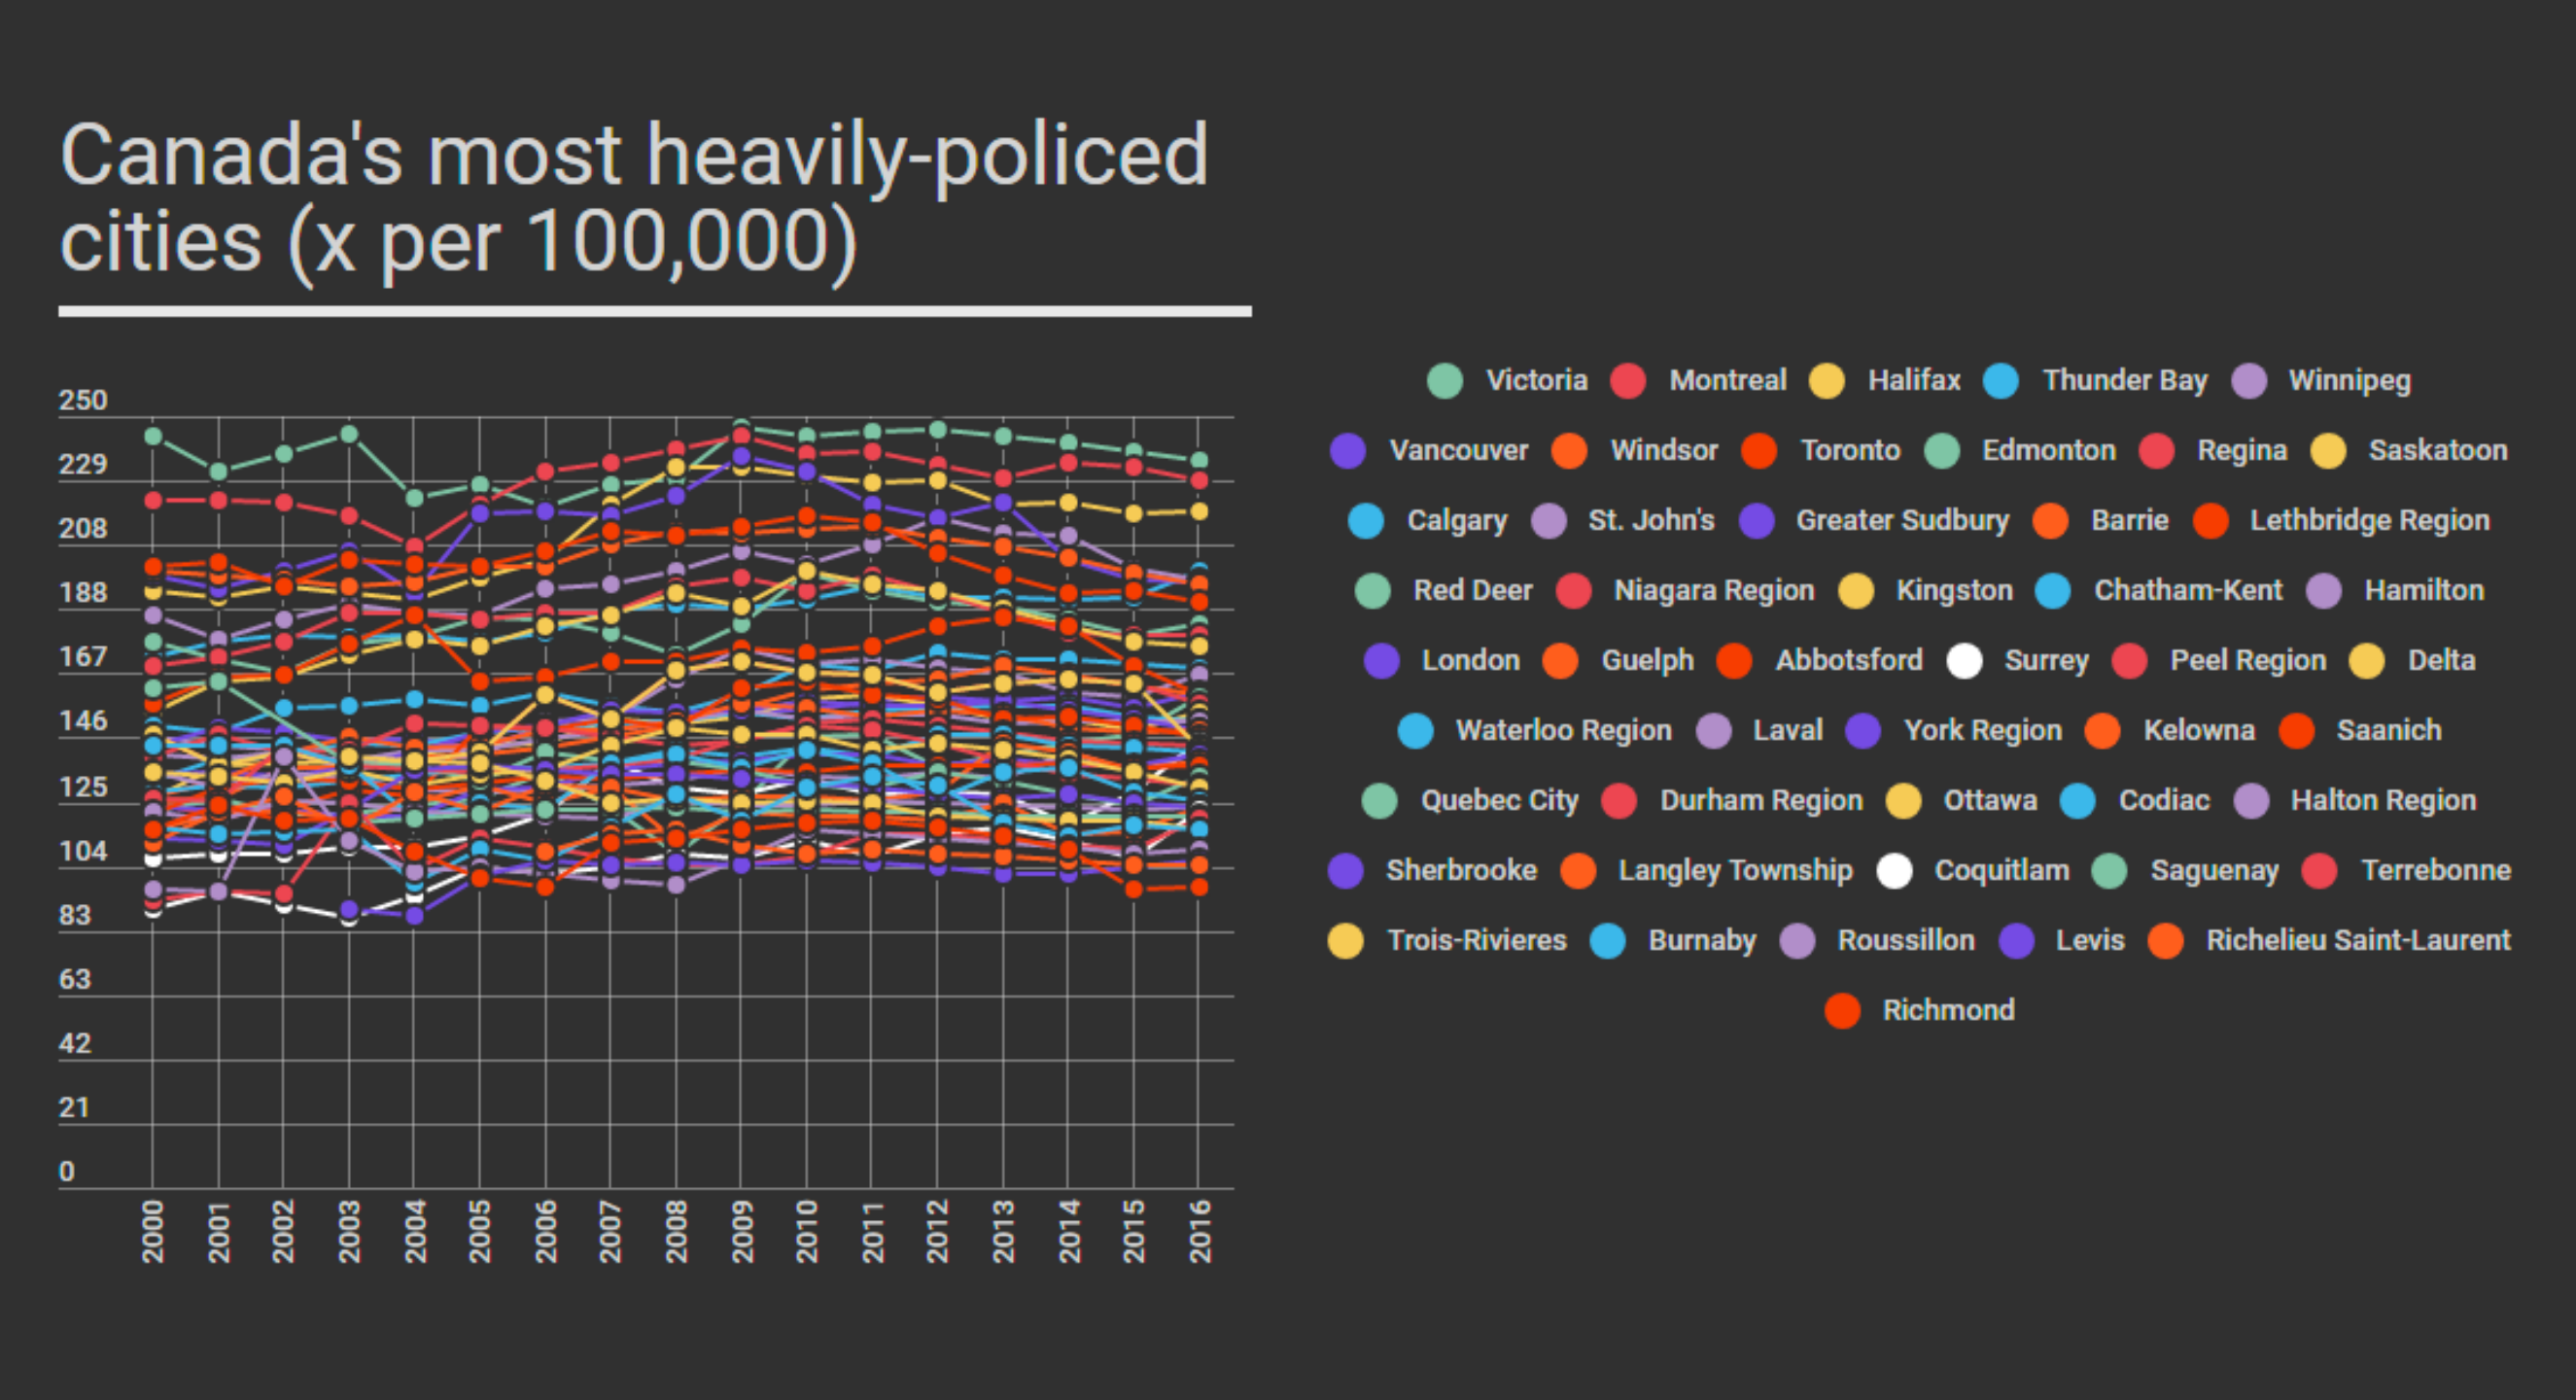
\includegraphics[keepaspectratio]{hallofshame_figs/fig_43.png}}
\end{frame}

\end{document}
